% Created 2025-03-31 Mon 10:10
\documentclass[10pt]{article}
\usepackage{graphicx}
\usepackage{longtable}
\usepackage{wrapfig}
\usepackage{rotating}
\usepackage[normalem]{ulem}
\usepackage{amsmath}
\usepackage{amssymb}
\usepackage{capt-of}
\usepackage{hyperref}
\usepackage[newfloat]{minted}
\usepackage[a4paper, total={6.5in, 9in}]{geometry}
\usepackage{minted}
\setminted{breaklines}
\usepackage[utf8]{inputenc}
\renewcommand{\familydefault}{\sfdefault}
\usemintedstyle{vs}
\usepackage[most]{tcolorbox}
\usepackage{CJKutf8}
\usepackage{xurl}
\usepackage{fontawesome5}
\usepackage{hyperref}
\usepackage{graphicx}
\usepackage{float}
\newcommand{\gitlab}[1]{%
\href{#1}{GitLab \faGitlab}}
\author{Vincent Conus\thanks{vincent.conus@protonmail.com}}
\date{2025-03-04}
\title{Setting up and using Xilinx KRIA KV260 and KR260\\\medskip
\large \begin{CJK}{UTF8}{min}南山大学\end{CJK}}
\hypersetup{
 pdfauthor={Vincent Conus},
 pdftitle={Setting up and using Xilinx KRIA KV260 and KR260},
 pdfkeywords={},
 pdfsubject={A report presenting how to use and set Xilinx's KRIA board},
 pdfcreator={Emacs 29.4 (Org mode 9.6.15)}, 
 pdflang={English}}
\begin{document}

\begin{titlepage}
\centering
{\LARGE Setting up and using Xilinx KRIA KV260 and KR260 \par }
\vspace{5mm}
{\large \begin{CJK}{UTF8}{min}南山大学\end{CJK} \par}
\vspace{1cm}
{\large 2025-03-04 \par}
\vspace{2cm}
{\large Vincent Conus -  Source available at \gitlab{https://gitlab.com/sunoc/xilinx-kria-kv260-documentation} \par}
\vspace{3cm}
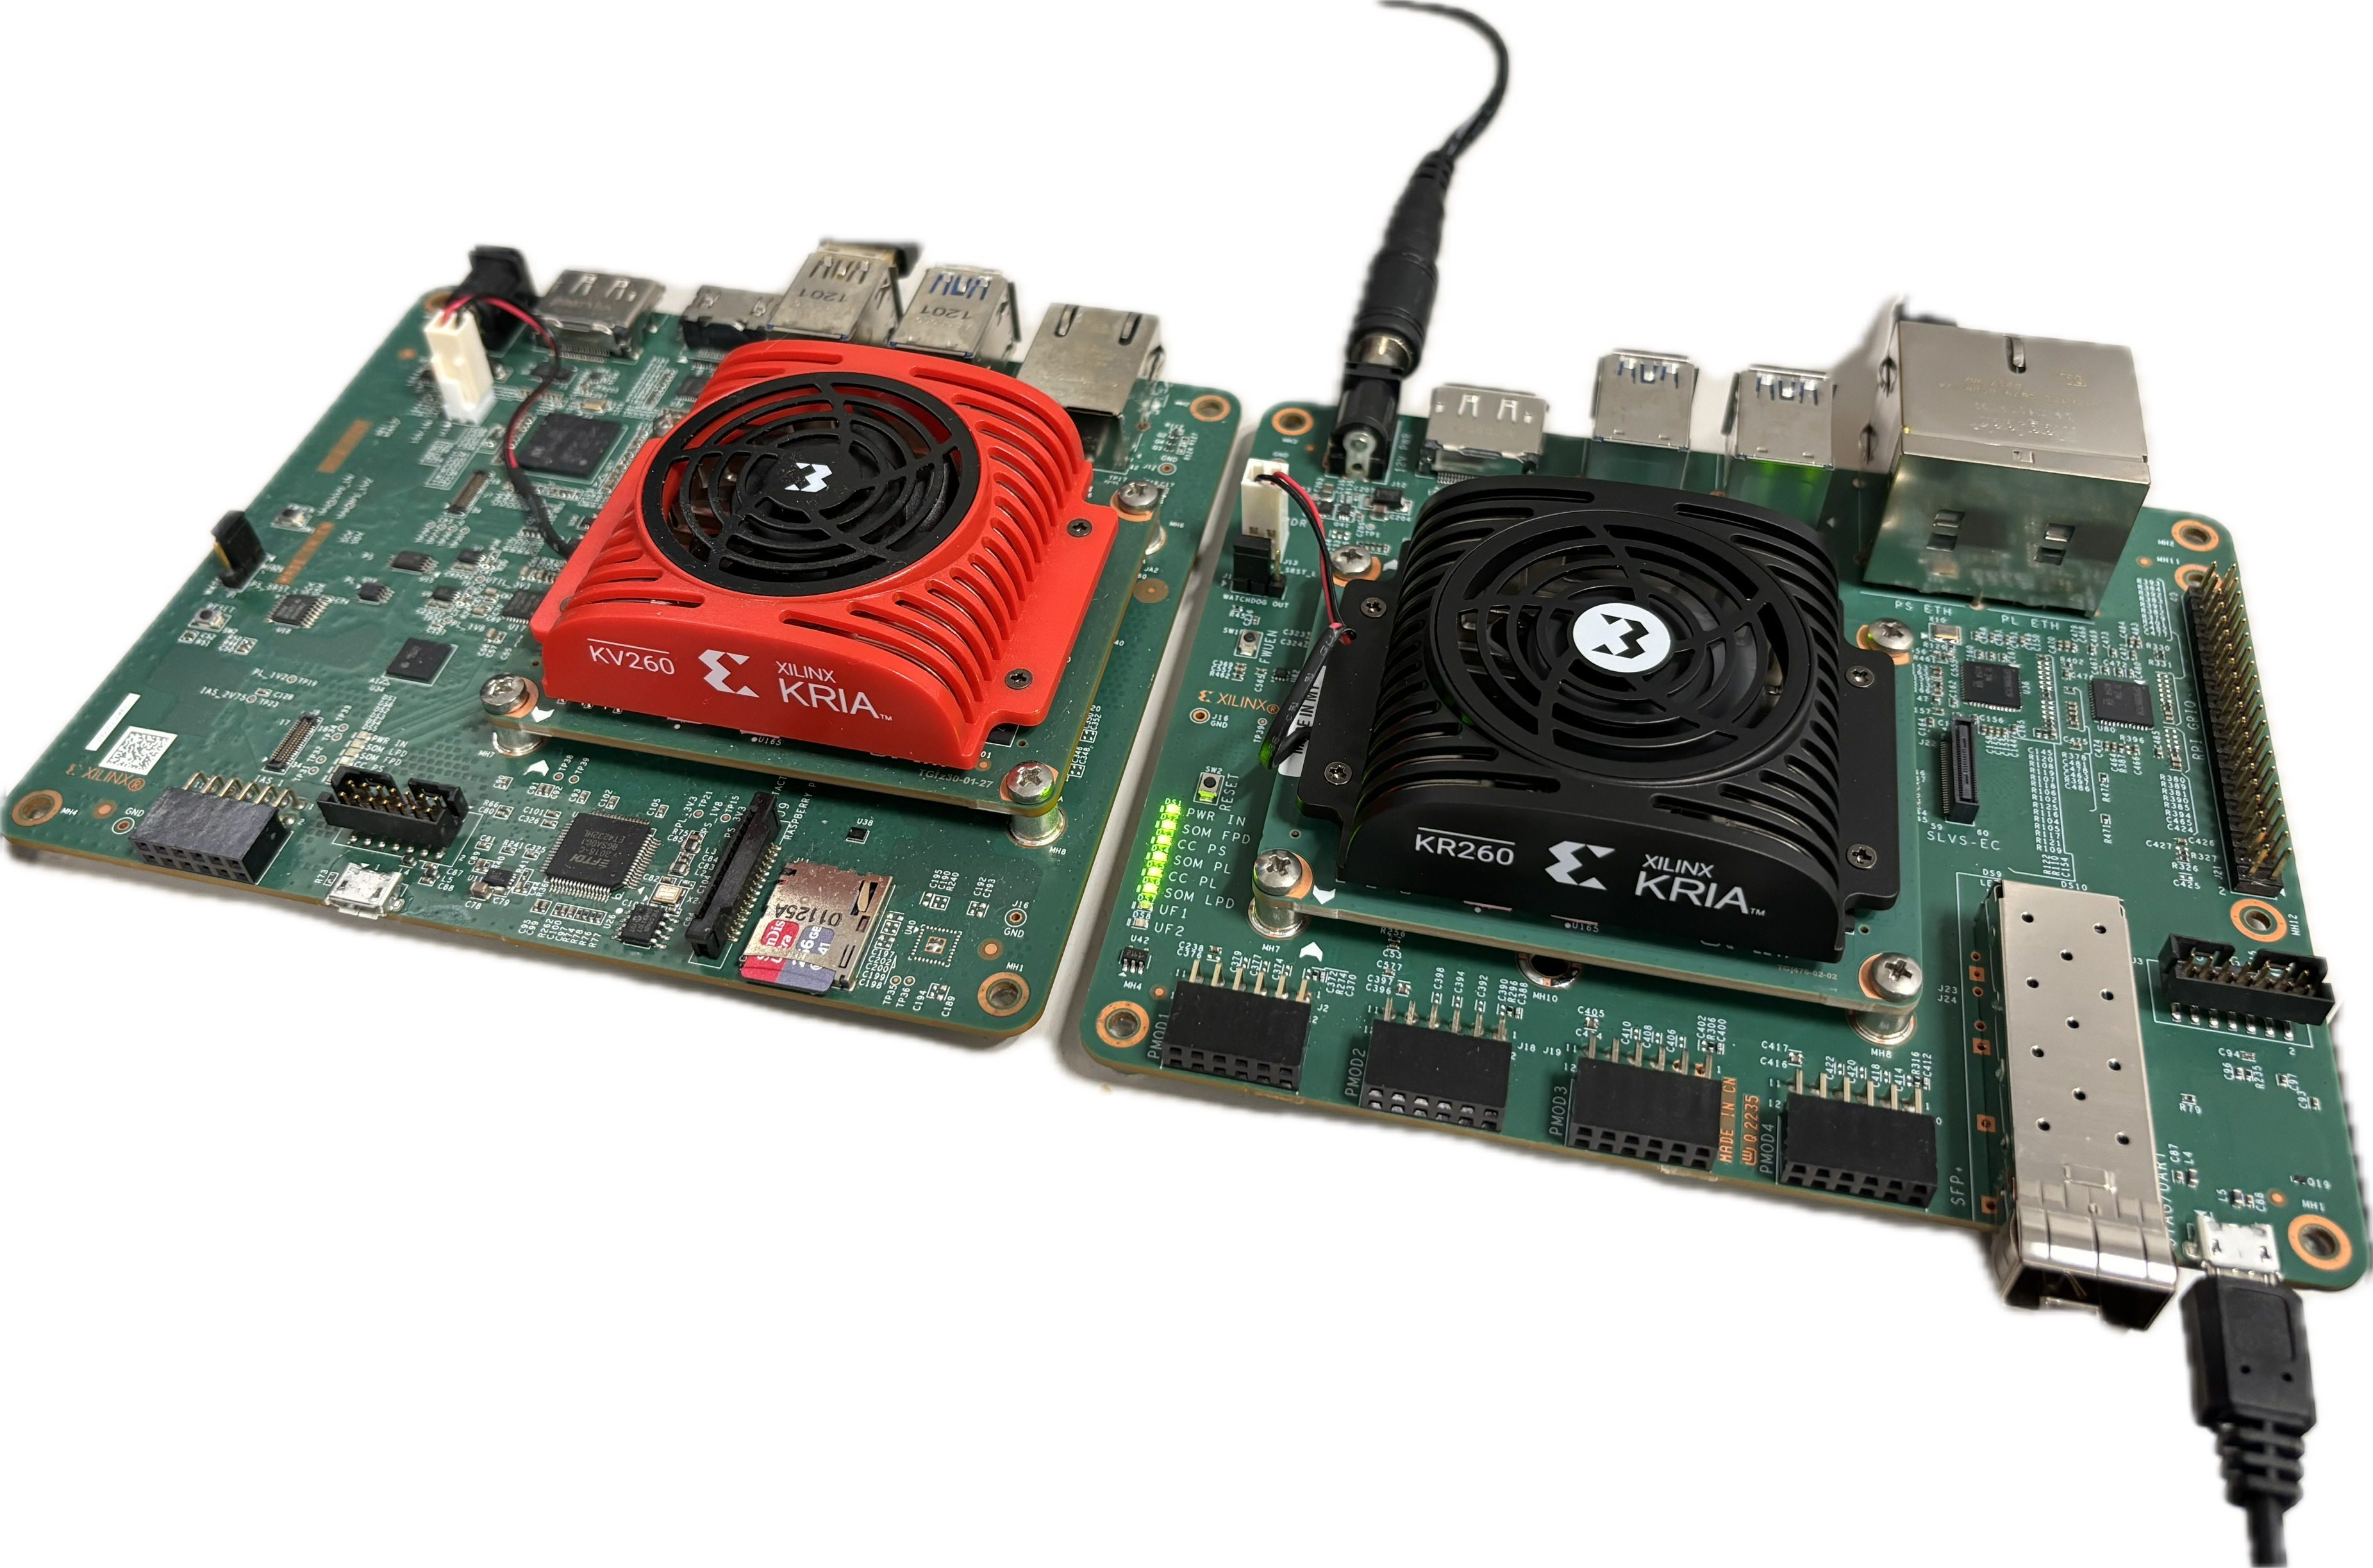
\includegraphics[width=0.8\textwidth]{./img/boards}\end{titlepage}
\tableofcontents
\pagebreak
\section{Introduction \& motivation}
\label{sec:org2fc766a}
This guide will present how to setup and use Xilinx's KRIA boards, in particular
for running ROS2 on a host Ubuntu system, as well as for deploying
micro-ROS\cite{Belsare2023} as a firmware on the micro-controller part of this board's chip.

The use of this device in particular is interesting because of the presence of a
SoC comprising both a general purpose ARM core (Cortex A53), capable of running
a Linux distribution, as well as another ARM core, real-time enabled, capable to
run a RTOS (Cortex R5F). The figure \ref{fig:org8ecc0fa} below shows a schematic view of the
overall system we are trying to archive.

\begin{figure}[htbp]
\centering
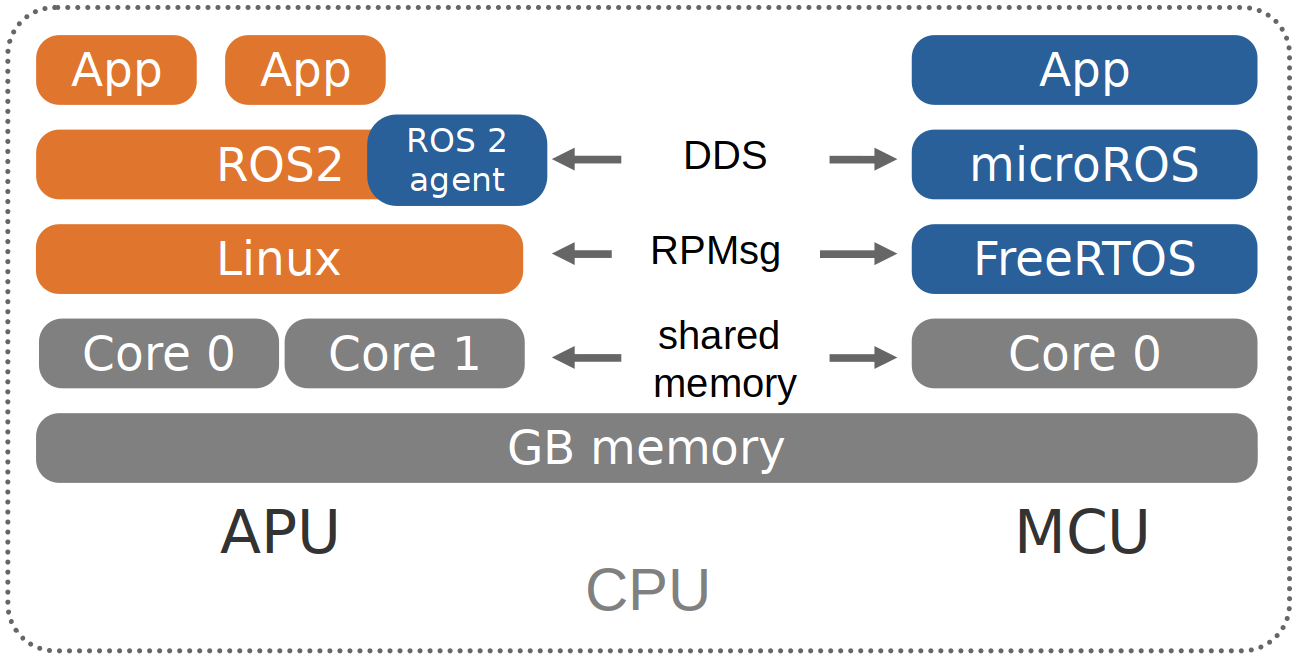
\includegraphics[width=.6\textwidth]{img/map.png}
\caption{\label{fig:org8ecc0fa}The Linux and ROS2 environment (orange) will communicate with the real-time, FreeRTOS and micro-ROS side (blue) using RPMsg (shared memory).}
\end{figure}

This document will give a step-by-step, chapter by chapter indication on how to go from a new board
to a system ready to be used for testing internal communication for ROS, between both types of cores
using the SoC shared memory.

\pagebreak
\section{Boot firmware update}
\label{sec:org8d80ad6}
The goal for the Linux side of the deployment is to
have the latest LTS version of Ubuntu up and running.

In order to be able to boot such a newer version of Linux, the
boot image of the board must first be updated.

The procedure is available in the official documentation\footnote{\url{https://docs.xilinx.com/r/en-US/ug1089-kv260-starter-kit/Firmware-Update}},
but I will present it step by step here.

\subsection{Getting the new firmware}
\label{sec:org270b07d}
A 2022.2 version of the board firmware is best in order to run the latest
version of Ubuntu or PetaLinux properly.

The image download link can be obtained at the Atlassian page\footnote{\url{https://xilinx-wiki.atlassian.net/wiki/spaces/A/pages/1641152513/Kria+SOMs+Starter+Kits\#K26-Boot-Firmware-Updates}} on the topic,
in the table detailing what version is best suited for which board.

In our case, we want to access this\footnote{\url{https://www.xilinx.com/member/forms/download/design-license-xef.html?filename=BOOT-k26-starter-kit-20230516185703.bin}} page. AMD login will be asked, then
download of firmware can be done.

\subsection{Reaching the board recovery tool}
\label{sec:orgd774340}
Now the firmware \texttt{.bin} image is available\footnote{Something that looks like \texttt{BOOT-k26-starter-kit-20230516185703.bin}, at the time of writing this section.}, it is possible to update it using the
boards recovery tool. Here are the steps that must be taken in order to reach
this tool and update the board:

\begin{itemize}
\item Power off the board and hold the firmware update button (FWUEN) when powering back the board.
\item Connect the board to your machine via a Ethernet cable.
This will obviously cut you internet access, so you should be set for that.
\item In the case of the KR260, the bottom right port should be used, as seen in the
figure \ref{fig:org7cd581e} below.
\item Select the wired network as your connection (must be "forced", since it
doesn't have internet access). To do so, you should disable the IPv6, and set
the IPv4 as manual, as visible in the figure \ref{fig:org2fdcc99} hereafter.
\item Set a fixed IP address for your machine, in the \texttt{192.168.0.2/24}
range, except the specific \texttt{192.168.0.111}, which will be used by the
board, and \texttt{192.168.0.1} which is the DNS and gateway.
The netmask and gateway should also be respectively set to
\texttt{255.255.255.0} and \texttt{192.168.0.1}.
\item Unplug the board power cord again. Hold the firmware update button (FWUEN)
when powering back the board.
\item Using a web browser on your host machine, access \texttt{http://192.168.0.111}. Thou
shall now see the interface, as visible on the figure \ref{fig:orgd14518e} below. If
the page struggle to appear, you should try to un-plug and re-plug the
Ethernet cable.
\end{itemize}

\begin{figure}[htbp]
\centering
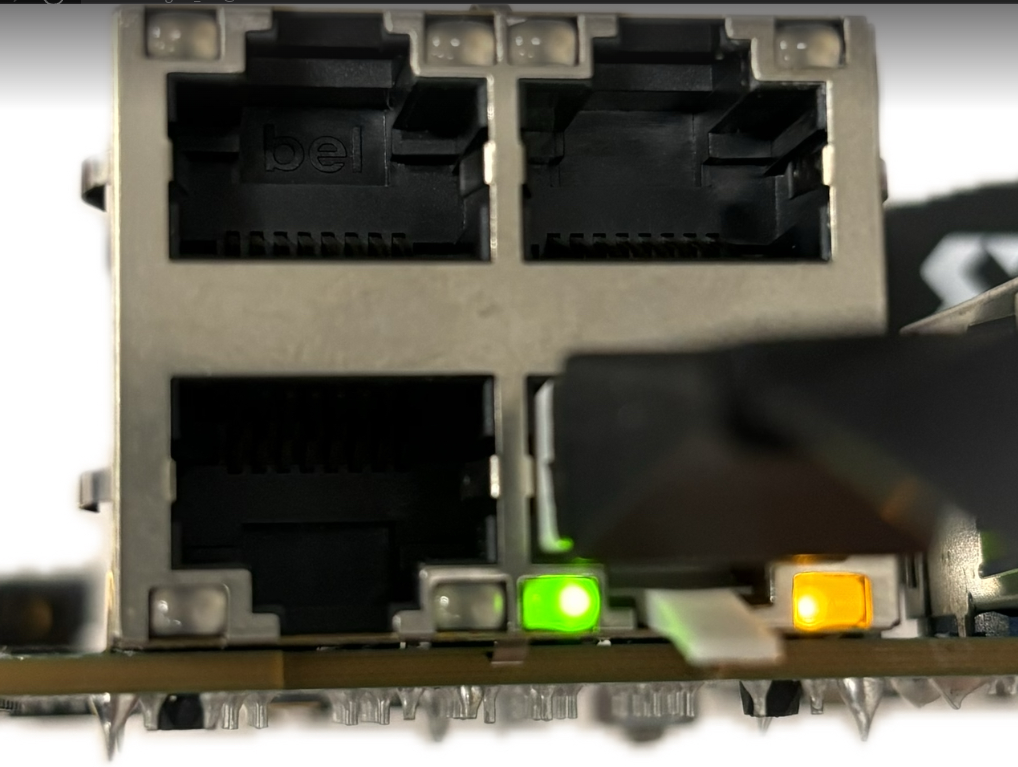
\includegraphics[width=.4\textwidth]{img/krport.png}
\caption{\label{fig:org7cd581e}Port to be used for the Ethernet Boot Recovery Tool access on the KR260 board.}
\end{figure}

\begin{figure}[htbp]
\centering
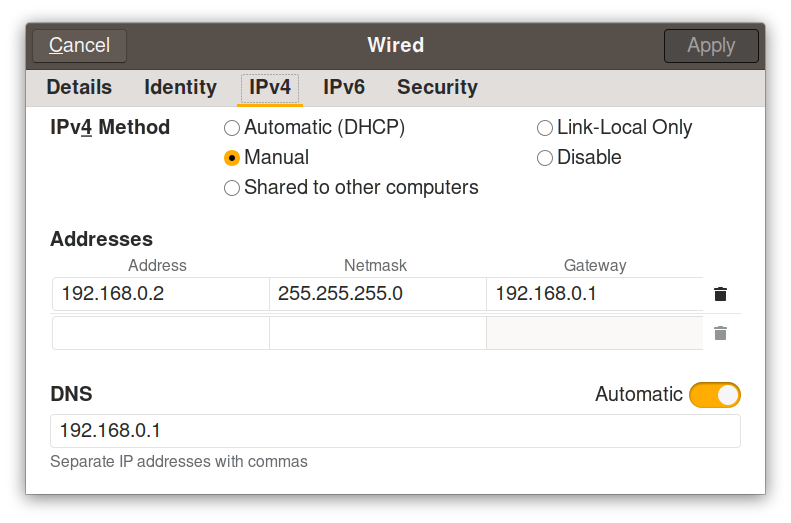
\includegraphics[width=.6\textwidth]{img/ipv4set.png}
\caption{\label{fig:org2fdcc99}IPv4 settings for accessing the Recovery Tool.}
\end{figure}

\begin{figure}[htbp]
\centering
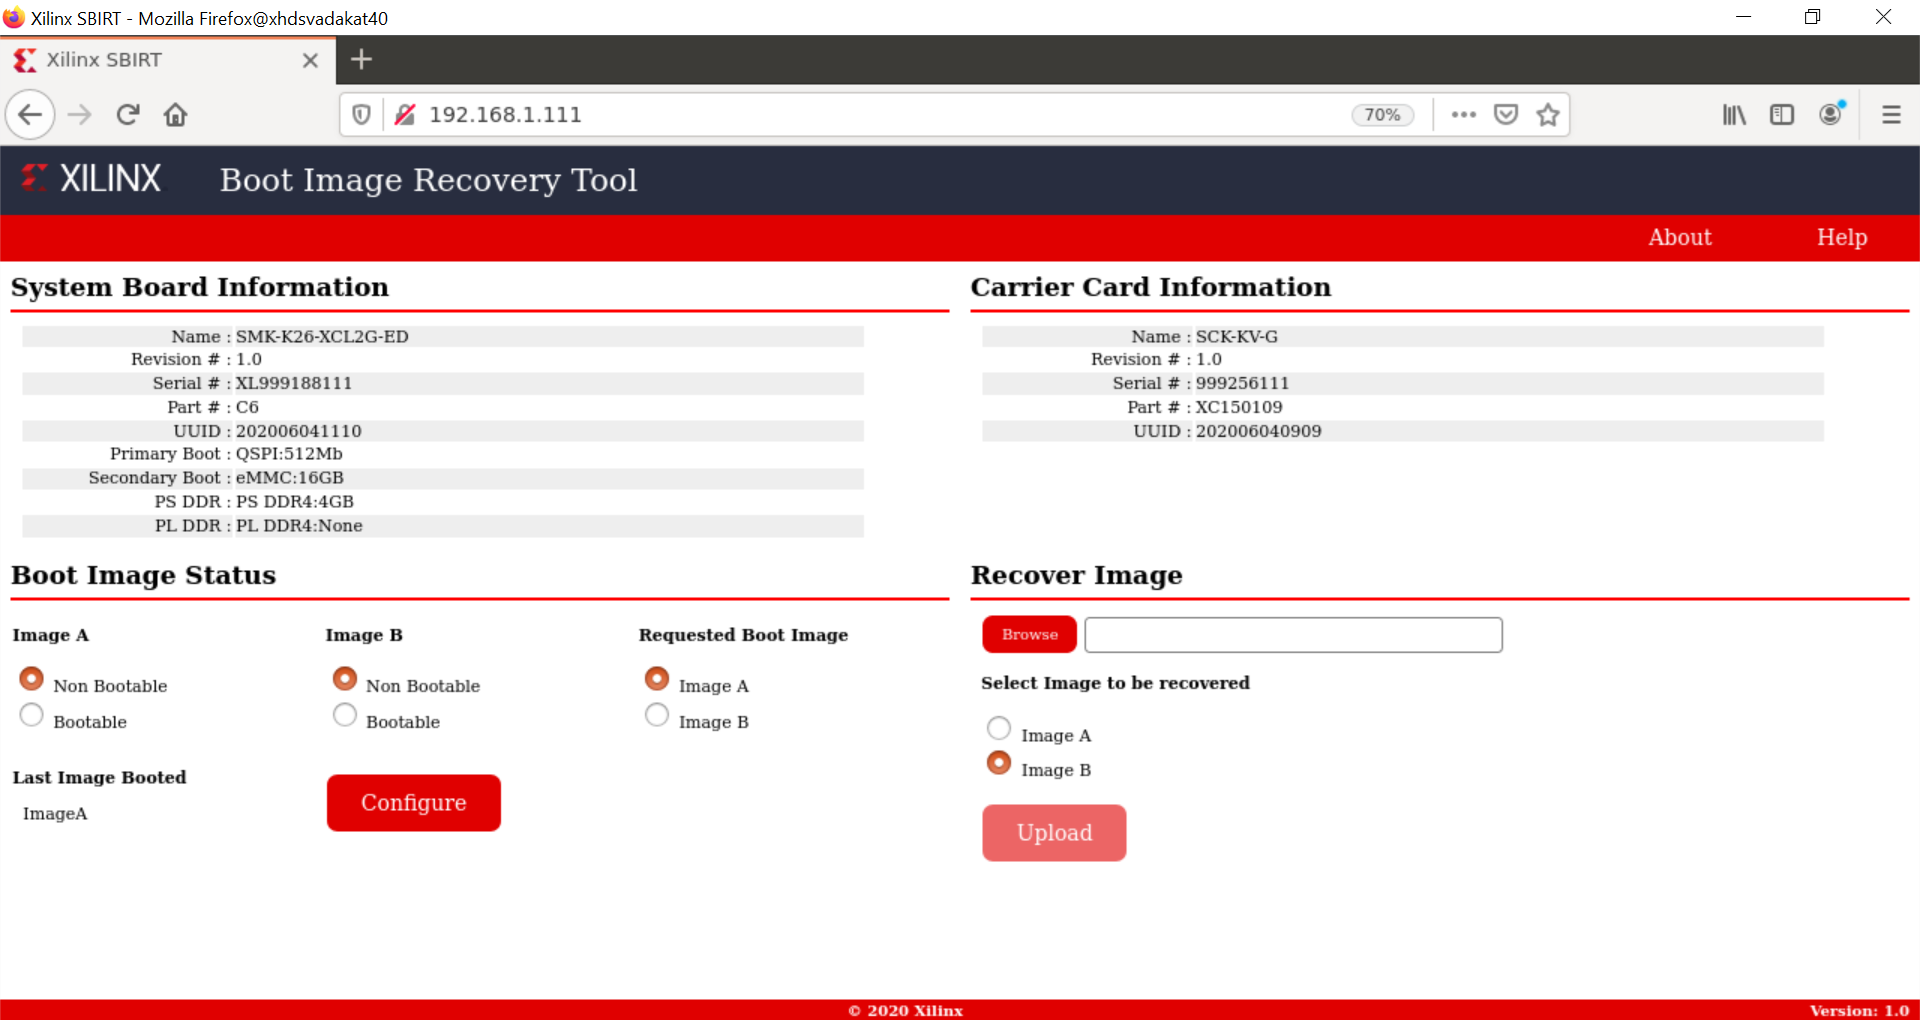
\includegraphics[width=1\textwidth]{img/recovery.png}
\caption{\label{fig:orgd14518e}The recovery tool for the board, access from Firefox. We can see board information at the center, and the tools to upload the firmware at the bottom of the page.}
\end{figure}

\subsection{Updating the boot firmware}
\label{sec:org8968555}
From this "recovery" page, it is possible to upload the \texttt{.bin} file downloaded previously onto
the board using the "Recover Image" section at the bottom right of the page.

The board can be re-booted afterwards.
\clearpage
\section{Installing Ubuntu LTS 22.04}
\label{sec:org8942216}
Withe the boot firmware being up-to-date, we can proceed to install a Linux distribution
on our Kria board. The step needed to archive a full installation of Ubuntu LTS 22.04
will be presented in this section\footnote{The same procedure should work for other versions of Ubuntu, as long as they
support the Kria board, but for this report and project, only the LTS 22.04 was tested
(as of 2023-08-30). 
\clearpage}. The figure \ref{fig:org119f9ab} below shows
where this operating system sits in the general system we are implementing.

\begin{figure}[htbp]
\centering
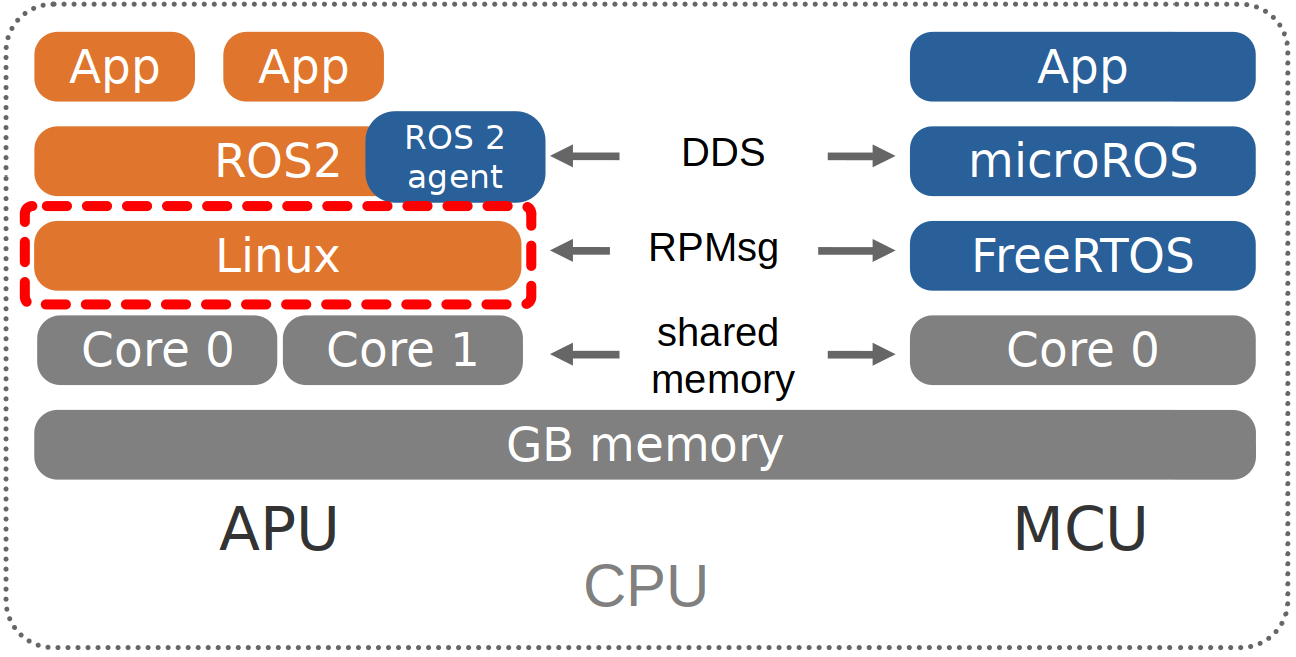
\includegraphics[width=.6\textwidth]{./img/map_linux.png}
\caption{\label{fig:org119f9ab}The Linux operating system (red border)runs on the APU (application, general purpose) side of the Kria board CPU. It is the base layer for the ROS2 system.}
\end{figure}

\subsection{Preparing and booting a Ubuntu 22.04 media}
\label{sec:orgcfaf314}
An \href{https://ubuntu.com/download/amd-xilinx}{official Ubuntu image} exists and is
provided by Xilinx, allowing the OS installation to be quick and
straightforward.
Ubuntu is a common and easy to use distribution. Furthermore,
it allows to install ROS2 as a package, which is most convenient and will be
done later in this guide.

Once the image has been downloaded at \href{https://ubuntu.com/download/amd-xilinx}{Canonical's page}
we can flash it onto the SD card, with the following instructions.

\begin{tcolorbox}[colback=red!5!white,colframe=red!75!black]
\textbf{DANGER}: The next part involve the \texttt{dd} command writing on disks!!!
As always with the dd command, thou have to be \textbf{VERY} careful on what arguments
thou give. Selecting the wrong disk will result on the destruction of
thy data !!
\uline{If you are unsure of what to do, seek assistance !}
\end{tcolorbox}

With the image available on thy machine and a SD card visible as \texttt{/dev/sda} device\footnote{Again, it is \uline{critical} to be 100$\backslash$% certain that you are working with
the correct device!}
one can simply run the \texttt{dd} command as follow to write the image to a previously formatted drive (here \texttt{/dev/sda}):

\begin{minted}[frame=single,framesep=2mm,baselinestretch=1.2,linenos,breaklines,fontsize=\footnotesize]{sh}
unxz iot-limerick-kria-classic-desktop-2204-20240304-165.img.xz
sudo dd if=iot-limerick-kria-classic-desktop-2204-20240304-165.img \
     of=/dev/sda status=progress bs=8M && sync
\end{minted}


Once the SD card is flashed and put back in the board, the micro-USB cable can be
connected from the PC to the board. It is then possible to
connect to the board in serial with an appropriate tool, for example \texttt{picocom},
as in the following example (the serial port that "appeared" was the \texttt{/dev/ttyUSB1} in this case\footnote{If two boards are plugged in for serial, the second one will be \texttt{/dev/ttyUSB5}, then \texttt{USB9} and so on.},
and the 115200 bit-rate is the default value for the board):

\begin{minted}[frame=single,framesep=2mm,baselinestretch=1.2,linenos,breaklines,fontsize=\footnotesize]{sh}
sudo picocom /dev/ttyUSB1 -b 115200
\end{minted}

In my case, I am using Emacs's \texttt{serial-term}:
\begin{minted}[frame=single,framesep=2mm,baselinestretch=1.2,linenos,breaklines,fontsize=\footnotesize]{sh}
M-x serial-term RET /dev/ttyUSB1 RET 115200 RET
\end{minted}

The default username / password pair for the very first boot is \texttt{ubuntu} and \texttt{ubuntu}. You will then be prompted to enter a new password.

Once logged in, it is typically easier and more convenient to connect the board
using SSH. When the board is connected to the network, it is possible to know
it's IP address with the \texttt{IP} command; then it is possible to connect to
the board with ssh, as follow (example, with the first command to be run on the board
and the second one on the host PC, both without the first placeholder hostnames):
\begin{minted}[frame=single,framesep=2mm,baselinestretch=1.2,linenos,breaklines,fontsize=\footnotesize]{sh}
kria# ip addr

host# ssh ubuntu@192.168.4.11
\end{minted}

\subsection{Network and admin setups}
\label{sec:org5c0d8c5}
This section presents a variety of extra convenience configurations
that can be used when setting-up the Kria board.

\subsubsection{Static IP address}
\label{sec:org719fc62}
A static IP can be set by writing the following
configuration into your \texttt{netplan} configuration file\footnote{The \texttt{chmod} command is used to update the permissions and silence some warnings}.

The name of the files might vary:
\begin{minted}[frame=single,framesep=2mm,baselinestretch=1.2,linenos,breaklines,fontsize=\footnotesize]{sh}
sudo chmod 0600 /etc/netplan/50-cloud-init.yaml 
sudo nano /etc/netplan/50-cloud-init.yaml
\end{minted}

You can then set the wanted IP as follow\footnote{For the routing part, it is key to have the \texttt{to} with a \texttt{'-'} in front of
it; and then the \texttt{via} without, but aligned with the \texttt{t}.}:
\begin{minted}[frame=single,framesep=2mm,baselinestretch=1.2,linenos,breaklines,fontsize=\footnotesize]{yaml}
network:
  renderer: NetworkManager
  version: 2
  ethernets:
    eth0:
      dhcp4: false
      addresses:
        - 192.168.11.107/24
      routes:
        - to: default
          via: 192.168.11.1
      nameservers:
        addresses: [192.168.11.1]
\end{minted}

Finally, the change in settings can be applied
as follow:

\begin{minted}[frame=single,framesep=2mm,baselinestretch=1.2,linenos,breaklines,fontsize=\footnotesize]{sh}
sudo netplan apply
\end{minted}

\subsubsection{[facultative] \texttt{root} password}
\label{sec:org366a372}
\begin{tcolorbox}[colback=orange!5!white,colframe=orange!75!black]
\textbf{WARNING}: Depending on your use-case, the setup presented in this
subsection can be a critical security breach as it remove the need for a root
password to access the admin functions of the board's Linux.
\uline{When in doubt, do not apply this configuration!!}
\end{tcolorbox}

If you board does not hold important data
and is available to you only, for test or development,
it might be convenient for the \texttt{sudo} tool to not ask for the
password all the time.
This change can be done by editing the sudoers file, and
adding the parameter \texttt{NOPASSWD}
at the \texttt{sudo} line:

\begin{minted}[frame=single,framesep=2mm,baselinestretch=1.2,linenos,breaklines,fontsize=\footnotesize]{sh}
sudo visudo

%sudo   ALL=(ALL:ALL) NOPASSWD: ALL
\end{minted}

Again, this is merely a convenience setup for devices staying at you desk. If
the board is meant to be used in any kind of production setup, a password
should be set for making administration tasks.

With all of these settings, you should be able to update the software of your
board without any issues:
\begin{minted}[frame=single,framesep=2mm,baselinestretch=1.2,linenos,breaklines,fontsize=\footnotesize]{sh}
sudo apt update
sudo apt dist-upgrade
sudo reboot now
\end{minted}

\subsubsection{Adding Xilinx specific repositories}
\label{sec:org8c70176}
The following commands will add \texttt{PPA} repositories that are specific for Xilinx boards using Ubuntu.
It is then possible to update the package list and eventually upgrade to some new packages.
\begin{minted}[frame=single,framesep=2mm,baselinestretch=1.2,linenos,breaklines,fontsize=\footnotesize]{sh}
sudo add-apt-repository ppa:ubuntu-xilinx/updates
sudo add-apt-repository ppa:xilinx-apps/ppa
sudo apt update
sudo apt upgrade
\end{minted}

\subsubsection{[facultative] Installing Docker}
\label{sec:org4382d2d}
It is possible to have a version of Docker installed simply by using the available repository,
but since we are on Ubuntu, a PPA is available from Docker in order to have the most up-to-date version.

Following \href{https://docs.docker.com/engine/install/ubuntu/\#install-using-the-repository}{the official documentation}, the following steps can be taken to install the latest version of
Docker on a Ubuntu system. The last command is meant to test the install.
If everything went smoothly, you should see something similar to what is presented
in the figure \ref{fig:org473894e} below, after the commands:

\begin{minted}[frame=single,framesep=2mm,baselinestretch=1.2,linenos,breaklines,fontsize=\footnotesize]{sh}
sudo apt-get update
sudo apt-get install ca-certificates curl
sudo install -m 0755 -d /etc/apt/keyrings
curl -fsSL https://download.docker.com/linux/ubuntu/gpg | \
    sudo gpg --dearmor -o /etc/apt/keyrings/docker.gpg

sudo chmod a+r /etc/apt/keyrings/docker.gpg

echo \
    "deb [arch="$(dpkg --print-architecture)" \
  signed-by=/etc/apt/keyrings/docker.gpg] \
  https://download.docker.com/linux/ubuntu \
  "$(. /etc/os-release && \
         echo "$VERSION_CODENAME")" stable" | \
    sudo tee /etc/apt/sources.list.d/docker.list > /dev/null

sudo apt-get update
sudo apt-get install docker-ce docker-ce-cli \
     containerd.io docker-buildx-plugin docker-compose-plugin
sudo usermod -aG docker $USER
newgrp docker

docker run hello-world
\end{minted}

\begin{figure}[htbp]
\centering
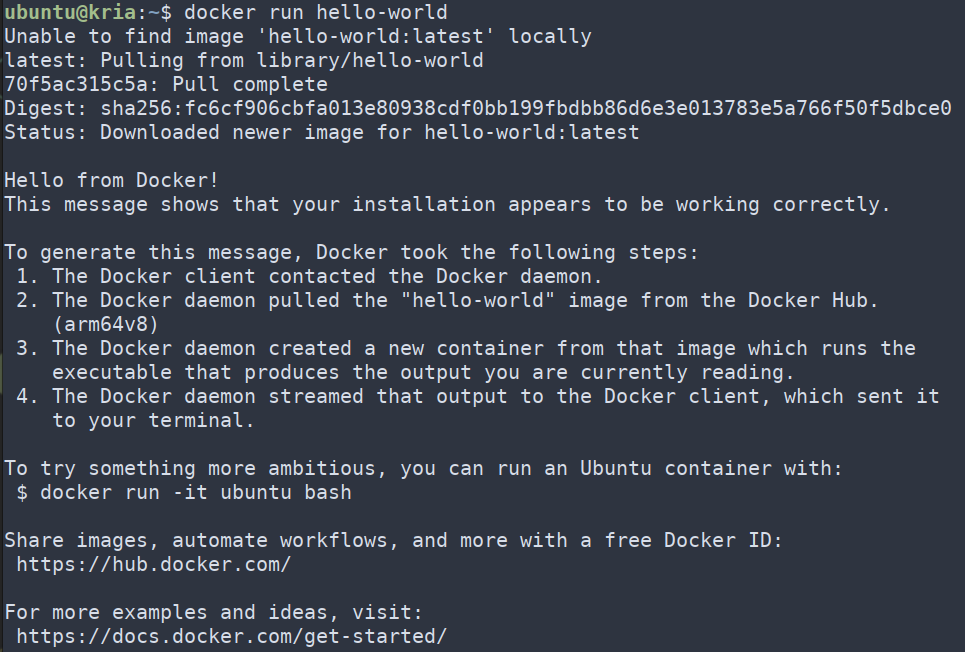
\includegraphics[width=.7\textwidth]{img/hello-docker.png}
\caption{\label{fig:org473894e}The return of a successful run of the \texttt{hello world} test Docker container.}
\end{figure}

\subsubsection{[recommended] Purging \texttt{snap}}
\label{sec:org992e1b0}
As the desktop-specific software are not used at all in the case
of our project, there are some packages that can be purges in order for the
system to become more lightweight.

In particular, the main issue with Ubuntu systems is the forced integration of
Snap packages. Here are the command to use in order to remove all of that.
These steps take a lot of time and need to be executed in that specific order\footnote{The \texttt{snap} packages depends on each others. Dependencies
cannot be remove before the package(s) that depends on them,
thus the specific delete order.},
but the system fan runs sensibly slower without all of this stuff.

Note that this all process is rather slow and can take up to 30min to complete.
\begin{minted}[frame=single,framesep=2mm,baselinestretch=1.2,linenos,breaklines,fontsize=\footnotesize]{sh}
sudo systemctl disable snapd.service
sudo systemctl disable snapd.socket
sudo systemctl disable snapd.seeded.service

sudo snap list #show installed package, remove them all:
sudo snap remove --purge firefox
sudo snap remove --purge gnome-3-38-2004
sudo snap remove --purge gnome-42-2204
sudo snap remove --purge gtk-common-themes
sudo snap remove --purge snapd-desktop-integration
sudo snap remove --purge snap-store
sudo snap remove --purge bare
sudo snap remove --purge core20
sudo snap remove --purge core22
sudo snap remove --purge snapd
sudo snap list # check that everything is uninstalled

sudo rm -rf /var/cache/snapd/
sudo rm -rf ~/snap
sudo apt autoremove --purge snapd

# check once more that there is no more snap on the system
systemctl list-units | grep snapd 
\end{minted}

\subsubsection{[facultative] Other unused heavy packages}
\label{sec:org29f843e}
Some other pieces of software can safely be removed since the desktop is
not to be used.
\begin{minted}[frame=single,framesep=2mm,baselinestretch=1.2,linenos,breaklines,fontsize=\footnotesize]{sh}
sudo apt-get autoremove --purge yaru-theme-icon \
     fonts-noto-cjk yaru-theme-gtk vim-runtime \
     ubuntu-wallpapers-jammy humanity-icon-theme

sudo apt-get autoclean
sudo reboot now
\end{minted}

\subsubsection{[facultative] Slow boot services to disable}
\label{sec:orge179022}
These packages (in particular the first one) are taking up a LOT of time at boot while providing no benefits\footnote{The CUPS and Docker services will be activated when used instead of during boot time.}.

It is possible to disable them as follow:
\begin{minted}[frame=single,framesep=2mm,baselinestretch=1.2,linenos,breaklines,fontsize=\footnotesize]{sh}
sudo systemctl disable systemd-networkd-wait-online.service
sudo systemctl disable NetworkManager-wait-online.service
sudo systemctl disable cups.service
sudo systemctl disable docker.service
sudo systemctl disable containerd.service
sudo systemctl disable cloud-init-local.service
\end{minted}

Additional, potentially unused services can be found using the very handy command:
\begin{minted}[frame=single,framesep=2mm,baselinestretch=1.2,linenos,breaklines,fontsize=\footnotesize]{sh}
sudo systemd-analyze blame
\end{minted}

\subsubsection{[facultative] Adding a swap partition}
\label{sec:org5fa59f8}
This part is very optional, in particular as it might slow down a bit the
boot time of the board (\textasciitilde{}2s), however it might become handy to have swap memory
available to avoid system failure under heavy use.

This whole procedure must be done externally, with the board system SD card
mounted on a host PC as an external volume.  As it is highly platform dependant,
I will not give a detailed explanation on how to do it, yet here are the key
points that should be done:
\begin{itemize}
\item Shutdown the Kria board, take out the SD card and put it in a host machine.
\item Make sure the disk is visible.
\item Make sure all volumes are \textbf{unmounted}.
\item Resize the main \texttt{root} partition (\textbf{not} the \texttt{boot}) so a space the size of the
wanted swap is free \textbf{after} the partition. You'd want something around 1GB.
\item In the empty space, create a new partition, which type is "linux swap".
\item Find and take note of the UUID of the new partition. This is useful hereafter.
\item \texttt{sync}
\item Un-mount everything, eject SD card.
\item Put the SD card back in the Kria.
\item Boot back to Ubuntu.
\end{itemize}

Going back on the Kria board Ubuntu after boot, the \texttt{/etc/fstab} file can be
updated as follow, modulo your actual UUID for the newly created partition, to
enable swap at boot time.
\begin{minted}[frame=single,framesep=2mm,baselinestretch=1.2,linenos,breaklines,fontsize=\footnotesize]{sh}
sudo -s
echo "UUID=8b13ed05-a91d-4x50-a44a-e654a0c67a2c none   swap    sw      0       0" >> /etc/fstab
reboot now
\end{minted}

\subsubsection{[OLD] Enabling \texttt{remoteproc} with Device-Tree patching}
\label{sec:org9efe15e}
One of the advantage of this Kria board, as cited previously, is the presence of
multiple types of core (APU, MCU, FPGA) on the same chip.

The part in focus in this guide is the usage of both the APU, running
a Linux distribution and ROS2; and the MCU, running FreeRTOS and micro-ROS.
Online available guides\footnote{A \href{https://speakerdeck.com/fixstars/fpga-seminar-12-fixstars-corporation-20220727}{slideshow} (JP) from Fixstar employees presents how to use the device
tree to enable the communication between the cores.} \textsuperscript{,}\,\footnote{A \href{https://zenn.dev/ryuz88/articles/kv260\_setup\_memo\_ubuntu22 }{blog post} (JP) shows all major steps on how to enable the \texttt{remoteproc}.} also provide information on how to deploy these types
of systems and enabling \texttt{remoteproc} for the Kria board, but this guide
will show a step-by-step, tried process to have a heterogeneous system
up and running.

The communication between both side is meant to be done using shared memory, but
some extra setup is required in order to be running the real-time firmware, in particular
for deploying micro-ROS on it.

As a first step in that direction, this section of the report
will present how to setup and use as an example firmware that utilizes the
\texttt{remoteproc} device in Linux in order to access shared memory
and communicate with the real-time firmware using the RPMsg system.

The communication system and interaction from the Linux side towards the real-time capable core
is not enabled by default within the Ubuntu image provided by Xilinx.

In that regard, some modification of the device tree overlay (DTO) is required in order to have
the \texttt{remoteproc} system starting.

\begin{enumerate}
\item Patching the device tree for RPMsg (standard, kernel space mode)
\label{sec:org254b5c6}
Firstly, we need to get the original firmware device tree, converted
into a readable format (DTS):

\begin{minted}[frame=single,framesep=2mm,baselinestretch=1.2,linenos,breaklines,fontsize=\footnotesize]{sh}
sudo dtc /sys/firmware/fdt 2> /dev/null > system.dts
\end{minted}

Then, a custom-made patch file can be downloaded and applied.
This file is available at the URL visible in the command below.

\begin{minted}[frame=single,framesep=2mm,baselinestretch=1.2,linenos,breaklines,fontsize=\footnotesize]{sh}
wget https://gitlab.com/sunoc/xilinx-kria-kv260-documentation/-/raw/main/src/system.patch

patch system.dts < system.patch
\end{minted}

\item Kernel \texttt{cmd} edit
\label{sec:orgb66d621}
As for the board to be able to reserve the correct amount of memory with the new settings, some
\texttt{cma} kernel configuration is needed\footnote{The overlapping memory will not prevent the board to boot,
but it disables the PWM for the CPU fan, which will then run at full speed, making noise.}:

\begin{minted}[frame=single,framesep=2mm,baselinestretch=1.2,linenos,breaklines,fontsize=\footnotesize]{sh}
sudo nano /etc/default/flash-kernel

LINUX_KERNEL_CMDLINE="quiet splash cma=512M cpuidle.off=1"
LINUX_KERNEL_CMDLINE_DEFAULTS=""
sudo flash-kernel
\end{minted}

Now the DTS file has been modified, one can regenerate the binary and place it on the \texttt{/boot} partition
and reboot the board:

\begin{minted}[frame=single,framesep=2mm,baselinestretch=1.2,linenos,breaklines,fontsize=\footnotesize]{sh}
dtc -I dts -O dtb system.dts -o user-override.dtb
sudo mv user-override.dtb /boot/firmware/
sudo reboot now
\end{minted}

\item Checking the patching
\label{sec:org8d3c555}
After rebooting, you can check the content of the \verb|remoteproc| system directory,
and a \texttt{remoteproc0} device should be visible, as follow:

\begin{minted}[frame=single,framesep=2mm,baselinestretch=1.2,linenos,breaklines,fontsize=\footnotesize]{sh}
ls /sys/class/remoteproc/
#  remoteproc0
\end{minted}

If it is the case, it means that the patch was successful and  that the remote processor is
ready to be used!
\pagebreak
\end{enumerate}

\subsubsection{[NEW] Enabling \texttt{remoteproc} for RPMsg in userspace with device-tree patch}
\label{sec:orgd7fe86b}
\begin{enumerate}
\item Kernel \texttt{cmd} edit
\label{sec:org022e592}
\begin{minted}[frame=single,framesep=2mm,baselinestretch=1.2,linenos,breaklines,fontsize=\footnotesize]{sh}
sudo nano /etc/default/flash-kernel

LINUX_KERNEL_CMDLINE="quiet splash cma=512M cpuidle.off=1"
LINUX_KERNEL_CMDLINE_DEFAULTS=""
sudo flash-kernel
\end{minted}

\item Patching the device tree for RPMsg in userspace
\label{sec:orga457a4a}
The  \texttt{system\_uio.patch}
\begin{minted}[frame=single,framesep=2mm,baselinestretch=1.2,linenos,breaklines,fontsize=\footnotesize]{bash}
sudo dtc /sys/firmware/fdt 2> /dev/null > system.dts

wget https://gitlab.com/sunoc/xilinx-kria-kv260-documentation/-/raw/main/src/system_uio.patch

patch system.dts < system_uio.patch

dtc -I dts -O dtb system.dts -o user-override.dtb
sudo mv user-override.dtb /boot/firmware/
sudo reboot now
\end{minted}

\item Checking the patching
\label{sec:org2253b6f}
If everything went correctly, on reboot and re-logging in the device, you should
see an output to the following command:
\begin{minted}[frame=single,framesep=2mm,baselinestretch=1.2,linenos,breaklines,fontsize=\footnotesize]{bash}
ls /sys/class/remoteproc/
\end{minted}
\end{enumerate}

\subsubsection{[DEPRECATED] Proxy and DNS}
\label{sec:org0b7542e}
\begin{tcolorbox}[colback=orange!5!white,colframe=orange!75!black]
\textbf{WARNING}: This setup is not needed anymore when using Honda-sensei's lab
wired network.
Adding it will cause the DNS to FAIL!
This section is kept as a reference.
\end{tcolorbox}
An issue that can occur when connecting the board to the internet is the
conflicting situation with the university proxy.
Indeed, as the network at Nanzan University requires to go through a proxy,
some DNS errors appeared.

In that case, it might become needed to setup the proxy for the school.

This can be done as follow, by exporting a https base proxy configuration
containing you AXIA credentials (this is specific to Nanzan University IT system),
then by consolidating the configuration for other types of connections in the \texttt{bashrc}:

\begin{minted}[frame=single,framesep=2mm,baselinestretch=1.2,linenos,breaklines,fontsize=\footnotesize]{sh}
export https_proxy="http://<AXIA_username>:\
       <AXIA_psw>@proxy.ic.nanzan-u.ac.jp:8080"

echo "export http_proxy=\""$https_proxy"\"" >> ~/.bashrc
echo "export https_proxy=\""$https_proxy"\"" >> ~/.bashrc
echo "export ftp_proxy=\""$https_proxy"\"" >> ~/.bashrc
echo "export no_proxy=\"localhost, 127.0.0.1,::1\"" >> ~/.bashrc
\end{minted}

Eventually the board can be rebooted in order for the setup to get applied cleanly.

\subsubsection{[DEPRECATED] Jupyter notebook setup}
\label{sec:org6f1b003}
Here are some instruction on how to install and setup Jupyter on a KRIA board,
accessing it remotely and using it for making data analysis.

The following commands will set the required packages and install Jupyter itself\footnote{Alongside other packages useful for data analysis, such as \texttt{pandas} or \texttt{numpy}.}:
\begin{minted}[frame=single,framesep=2mm,baselinestretch=1.2,linenos,breaklines,fontsize=\footnotesize]{sh}
sudo apt-get update && sudo apt-get install python3 python3-pip python3-venv python3-virtualenv

virtualenv myjupyter
source ./myjupyter/bin/activate
python3 -m pip install jupyter pandas numpy matplotlib scipy

sudo reboot now
\end{minted}

Then in a terminal on your host machine (not on the KRIA board), you can run the following command\footnote{In this example, the full \texttt{username@IP} is used, but a \texttt{.ssh/config} is also usable.} to bind local ports:
\begin{minted}[frame=single,framesep=2mm,baselinestretch=1.2,linenos,breaklines,fontsize=\footnotesize]{sh}
ssh -L 8888:localhost:8888 ubuntu@192.168.11.107
\end{minted}

Then on the opened SSH shell to the KRIA board:
\begin{minted}[frame=single,framesep=2mm,baselinestretch=1.2,linenos,breaklines,fontsize=\footnotesize]{sh}
source ./myjupyter/bin/activate
jupyter notebook
\end{minted}

From there, it is possible to use the displayed URL (something that looks like
\texttt{http://localhost:8888/tree?token}) to access the remote Notebook system from a local web browser.
It is possible to do so with \texttt{localhost} since we have the \texttt{ssh} port map connection going on.

Eventually creating Notebooks and stuff, it is possible to obtain a situation like shown in the figure \ref{fig:org38d0cff} below.

\begin{figure}[htbp]
\centering
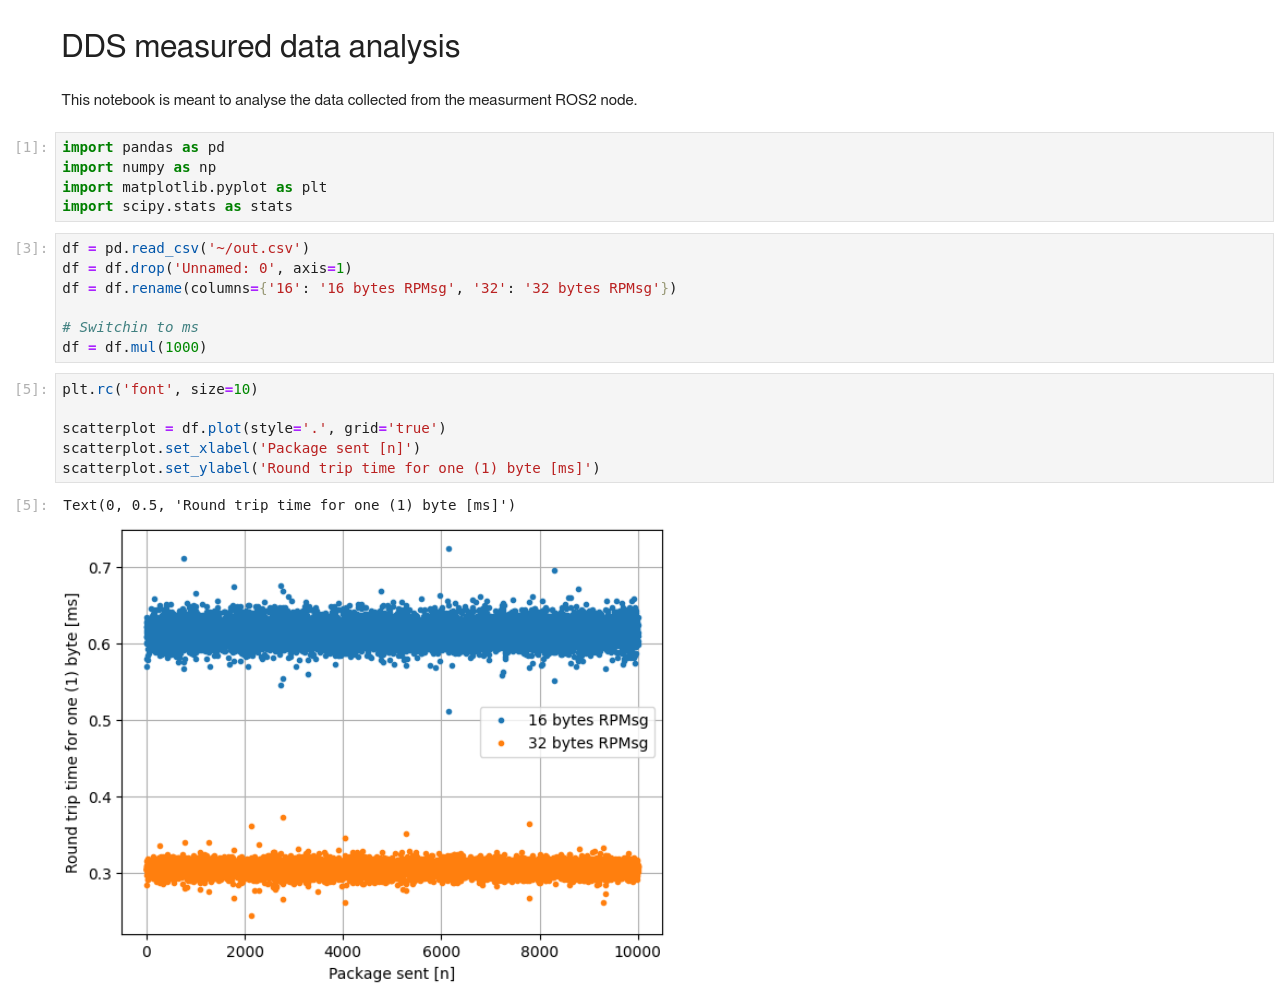
\includegraphics[width=.6\textwidth]{img/jupyter.png}
\caption{\label{fig:org38d0cff}A test Jupyter Notebook for CSV data analysis.}
\end{figure}

\subsubsection{[TODO] Using a PetaLinux kernel in Ubuntu}
\label{sec:org0228528}
TBD

\subsection{RPMsg standalone evaluation}
\label{sec:orgf42947b}
\subsubsection{[TODO] RPMsg Cortex R5F demonstration firmware}
\label{sec:org50c0f75}
\subsubsection{RPMsg \texttt{echo\_test} software}
\label{sec:org8efd4fa}
In order to test the deployment of the firmware on the R5F side, and in particular
to test the RPMsg function, we need some program on the Linux side of the KRIA
board to "talk" with the real-time side.

Some source is provided by Xilinx to build a demonstration software that does
this purpose: specifically interact with the demonstration firmware.

Here are the steps required to obtain the sources, and build the program.

As a reminder, this is meant to be done on the Linux running on the
KRIA board, NOT on your host machine !

\begin{minted}[frame=single,framesep=2mm,baselinestretch=1.2,linenos,breaklines,fontsize=\footnotesize]{sh}
git clone https://github.com/Xilinx/meta-openamp.git
cd  meta-openamp
git checkout xlnx-rel-v2022.2
cd  ./recipes-openamp/rpmsg-examples/rpmsg-echo-test
make
sudo ln -s $(pwd)/echo_test /usr/bin/
\end{minted}

Once this is done, it it possible to run the test program from the KRIA board's Ubuntu
by running the \texttt{echo\_test} command.
\section{Building micro-ROS as a static library}
\label{sec:org180933a}
This section will present the way to build manually the micro-ROS system as static library
that can be used to port it to a different platform.

\subsection{Initial setup}
\label{sec:org1e8a820}
In this section, the goal is to build the micro-ROS library in order to be
able to integrate it's functions into our Cortex R5F firmware.

All of this should be done via cross-compiling on a host machine, however
it is most common in the guides about micro-ROS to build the firmware and libraries within a Docker,
so we can have access of the ROS environment without installing it permanently.

One can simply run this command to summon a ROS2 Docker\footnote{If Docker is not set up on your machine, you can follow the guide on \href{https://docs.docker.com/engine/install/ubuntu/}{the official website}.
When you can successfully run the "hello-world" container, you are good to go.} with the wanted version,
but first we also need to check the cross-compilation tools.

We are downloading the latest \texttt{arm-none-eabi} gcc compiler directly from the ARM website.

The cross-compilation tool can then be extracted, set as our \texttt{toolchain} variable,
then passed as a parameter when creating the Docker container:
\begin{minted}[frame=single,framesep=2mm,baselinestretch=1.2,linenos,breaklines,fontsize=\footnotesize]{sh}
pushd /home/$USER/Downloads
wget https://developer.arm.com/-/media/Files/downloads/gnu/13.2.rel1/binrel/arm-gnu-toolchain-13.2.rel1-x86_64-arm-none-eabi.tar.xz
tar -xvf arm-gnu-toolchain-13.2.rel1-x86_64-arm-none-eabi.tar.xz
popd

toolchain="/home/$USER/Downloads/arm-gnu-toolchain-13.2.Rel1-x86_64-arm-none-eabi/"


docker run -d --name ros_build -it --net=host \
       --hostname ros_build \
       -v $toolchain:/armr5-toolchain \
       --privileged ros:iron
\end{minted}

Now the container named \texttt{ros\_build} was created, it is possible to "enter" it, and having access
to the tools in it by running the following command that will open a \texttt{bash} shell in said container:
\begin{minted}[frame=single,framesep=2mm,baselinestretch=1.2,linenos,breaklines,fontsize=\footnotesize]{sh}
docker exec -it ros_build bash
\end{minted}

\subsection{Building the static library}
\label{sec:orgf81bce9}
Now we are in the ROS2 container, we can build the micro-ROS firmware as presented
in the \href{https://micro.ros.org/docs/tutorials/advanced/create\\\_custom\\\_static\\\_library}{dedicated micro-ROS guide}:
\#+BEGIN\textsubscript{SRC} sh
echo 127.0.0.1 \$HOSTNAME >> /etc/hosts
sudo apt update 
sudo apt-get -y install python3-pip $\backslash$
     wget $\backslash$
     nano

. /opt/ros/\$ROS\textsubscript{DISTRO}/setup.bash

mkdir microros\textsubscript{ws}
cd microros\textsubscript{ws}
git clone -b \$ROS\textsubscript{DISTRO} $\backslash$
    \url{https://github.com/micro-ROS/micro\_ros\_setup.git} $\backslash$
\clearpage
\section{ROS2 host system setup}
\label{sec:org46c7d9d}
This is focused on the ROS2 system being used on the Kria board as a base to run and / or build
micro-ROS components.

The installation of ROS2 as a system will be presented, with
two different ways of approaching the problem.

As for the previous section, the figure \ref{fig:org712a006} below shows what part
of the overall system we are talking about here.

\begin{figure}[htbp]
\centering
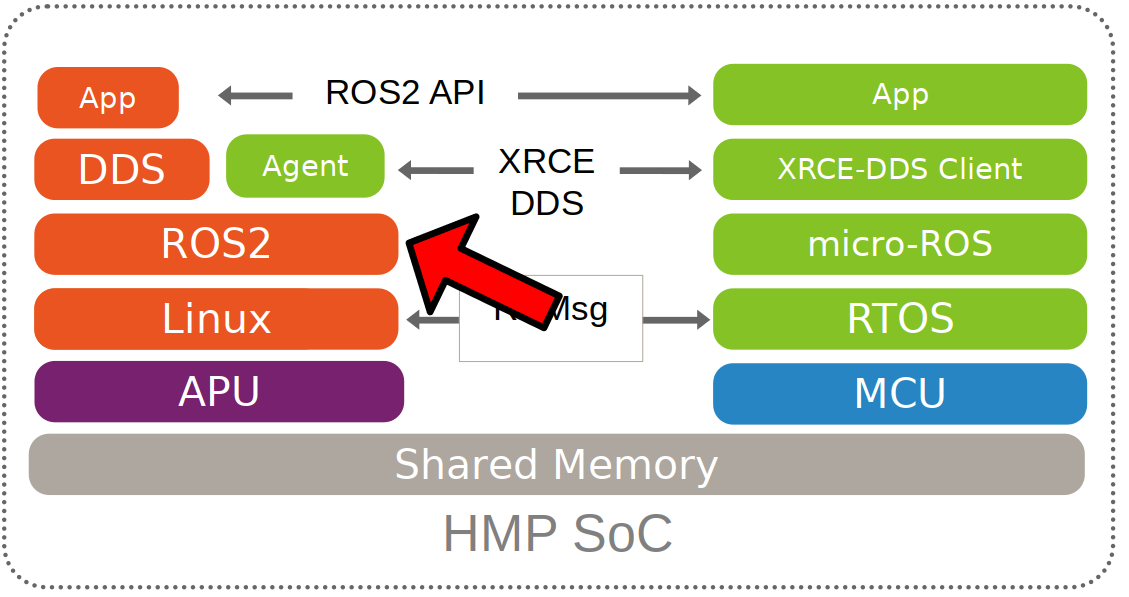
\includegraphics[width=.6\textwidth]{./img/map_ros.png}
\caption{\label{fig:org712a006}The ROS2 middle (red border) runs on top of the Linux, on the general-purpose core of the Kria board.}
\end{figure}

\begin{figure}[htbp]
\centering
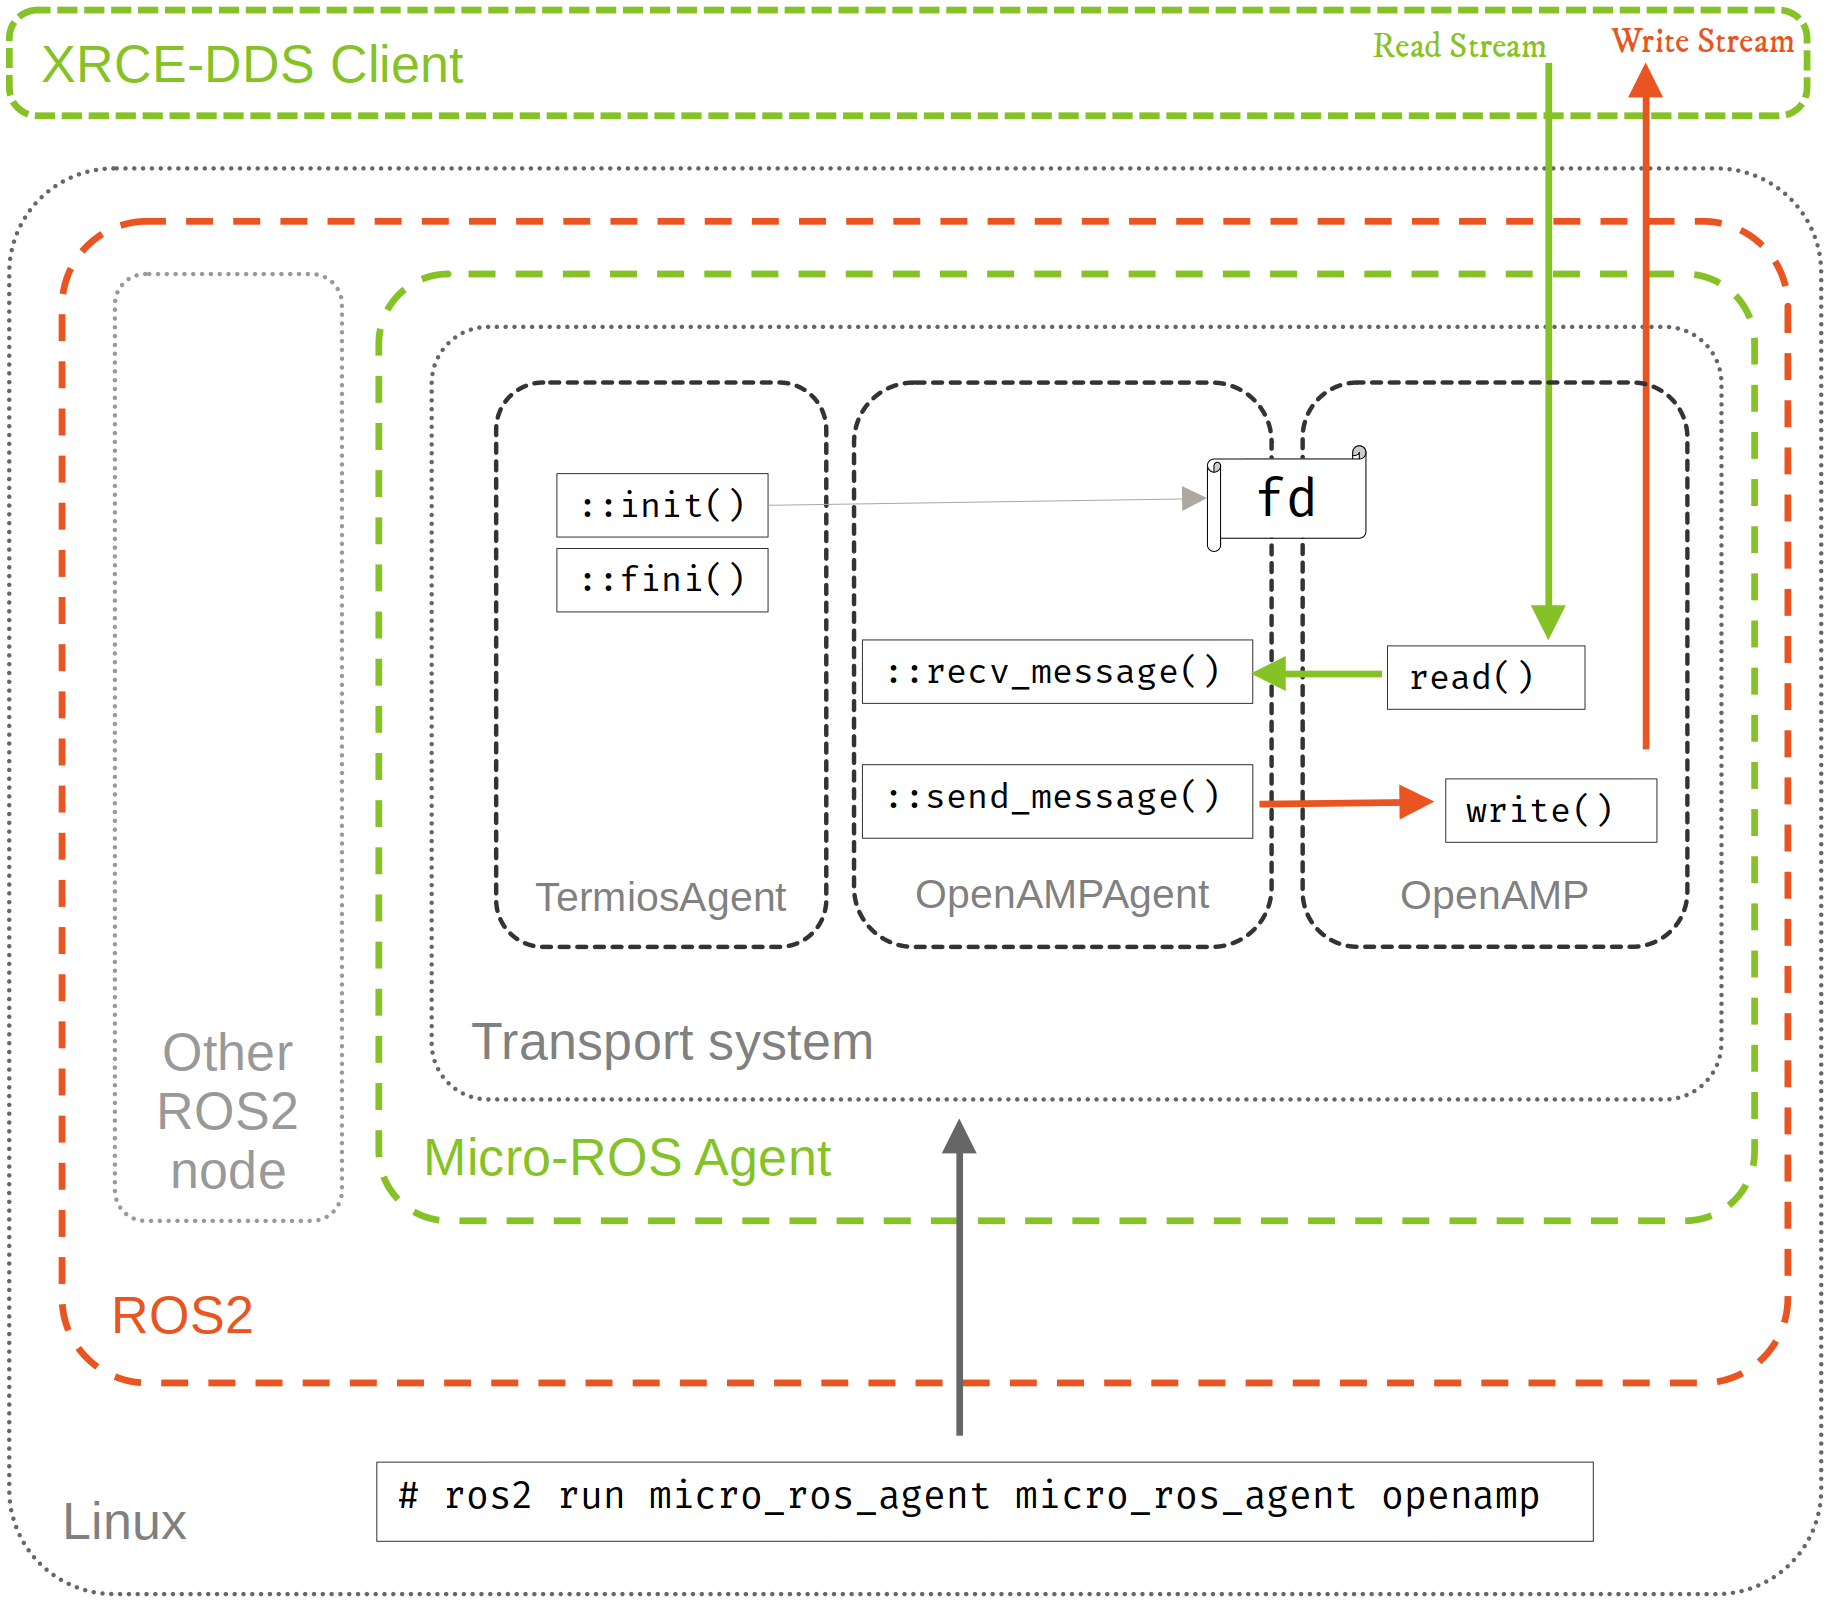
\includegraphics[width=.55\textwidth]{./img/agent_arch.png}
\caption{\label{fig:org1b4fba9}Methods architecture for the modified Agent node.}
\end{figure}

\subsection{On the host Linux ("bare-metal")}
\label{sec:org5225166}
Since an Ubuntu distribution is installed on the board, the installation of ROS2
can be done\footnote{As always, this configuration was tested solely on Ubuntu LTS 22.04,
with the ROS2 versions \texttt{Humble} and then \texttt{Iron} being deployed.
Other combination of versions should work as well, but they are not
tested for this guide. In case of doubt or problem, please refer to the official documentation.} in a standard way, using the repository.

An \href{https://docs.ros.org/en/humble/Installation/Ubuntu-Install-Debians.html}{official documentation} is provided with ROS2 themselves with a step-by-step guide on how to install
ROS2 on a Ubuntu system\{\}.
We will be following this guide here\footnote{The \texttt{curl} command from the guide does not work through the school proxy,
but the command \texttt{wget} used instead does work. The key is then moved to the correct spot with \texttt{mv}.}.

Firstly, we need to update the locals, enable the universe Ubuntu repository,
get the key and add the repository for ROS2. This can be done as follow:
\begin{minted}[frame=single,framesep=2mm,baselinestretch=1.2,linenos,breaklines,fontsize=\footnotesize]{sh}
locale  # check for UTF-8
sudo apt update && sudo apt install -y locales
sudo locale-gen en_US en_US.UTF-8
sudo update-locale LC_ALL=en_US.UTF-8 LANG=en_US.UTF-8
export LANG=en_US.UTF-8
locale  # verify settings

sudo apt install -y software-properties-common
sudo add-apt-repository universe
sudo apt update && sudo apt install -y curl wget

wget https://raw.githubusercontent.com/ros/rosdistro/master/ros.key
sudo mv ros.key /usr/share/keyrings/ros-archive-keyring.gpg
\end{minted}

Then, a thick one-liner is available to add the ROS2 repository to our system:
\begin{minted}[frame=single,framesep=2mm,baselinestretch=1.2,linenos,breaklines,fontsize=\footnotesize]{sh}
echo "deb [arch=$(dpkg --print-architecture) \
signed-by=/usr/share/keyrings/ros-archive-keyring.gpg] \
http://packages.ros.org/ros2/ubuntu $(. \
/etc/os-release && echo $UBUNTU_CODENAME) main" | \
    sudo tee /etc/apt/sources.list.d/ros2.list > /dev/null
\end{minted}

It is then possible to install ROS2\footnote{This command installs a complete "desktop" version of ROS2, containing many
useful package for our project.
If space is a constraint, different, less complete packages can be install.
Please refer to the official documentation about it.} as follow:
\begin{minted}[frame=single,framesep=2mm,baselinestretch=1.2,linenos,breaklines,fontsize=\footnotesize]{sh}
sudo apt update
sudo apt upgrade -y
sudo apt install -y ros-$ROS_DISTRO-desktop \
     ros-$ROS_DISTRO-ros-base \
     python3-argcomplete \
     ros-dev-tools
\end{minted}

Once installed, it is possible to test the system with a provided example.
You need to open two terminals and log wish SSH onto the board, then running
respectively:
\begin{minted}[frame=single,framesep=2mm,baselinestretch=1.2,linenos,breaklines,fontsize=\footnotesize]{sh}
source /opt/ros/$ROS_DISTRO/setup.bash
ros2 run demo_nodes_cpp talker
\end{minted}

And then:
\begin{minted}[frame=single,framesep=2mm,baselinestretch=1.2,linenos,breaklines,fontsize=\footnotesize]{sh}
source /opt/ros/$ROS_DISTRO/setup.bash
ros2 run demo_nodes_py listener
\end{minted}

You should be able to see the first terminal sending "Hello world" messages,
and the second one receiving then.

\subsection{In a container (Docker)}
\label{sec:orgcca2c49}
As containers are used to test and build micro-ROS configurations,
running ROS2 in a Docker  is a great way to have a reproducible configuration
of you system.

This part of the guide will present how to install Docker on the
Kria board and then how to use it to deploy the latest version of ROS2.
This section of the report assumes that Docker was installer on the target system.

The following commands will pull a ROS container, version \texttt{iron}, and name it \texttt{ros\_build}.

A key part for having access to the interfaces (serial) is the mapping of the whole \texttt{/dev}
range of devices from the host machine to the internal \texttt{/dev} of the container\footnote{This is an example and this situation can become a security issue. It would be a better practice
in a production environment to map only the devices that are actually in use.}.
With the second command, we can execute \texttt{bash} as a way to open a terminal to the "inside" the container:
\begin{minted}[frame=single,framesep=2mm,baselinestretch=1.2,linenos,breaklines,fontsize=\footnotesize]{sh}
docker run -d --name ros_agent -it --net=host -v \
       /dev:/dev --privileged ros:iron
docker exec -it ros_agent bash
\end{minted}

From there, it becomes possible to simply use ROS2 as you would for a bare-metal install,
and as presented in the section \ref{sec:org5225166} above:
\begin{minted}[frame=single,framesep=2mm,baselinestretch=1.2,linenos,breaklines,fontsize=\footnotesize]{sh}
source /opt/ros/$ROS_DISTRO/setup.bash

# Create a workspace and download the micro-ROS tools
mkdir microros_ws
cd microros_ws
git clone -b $ROS_DISTRO https://github.com/micro-ROS/\
    micro_ros_setup.git src/micro_ros_setup

# Update dependencies using rosdep
sudo apt update && rosdep update
rosdep install --from-paths src --ignore-src -y

# Install pip
sudo apt-get install python3-pip

# Build micro-ROS tools and source them
colcon build

# Download micro-ROS-Agent packages
source install/local_setup.bash
ros2 run micro_ros_setup create_agent_ws.sh

# Build step
ros2 run micro_ros_setup build_agent.sh

# Run a micro-ROS agent
ros2 run micro_ros_agent micro_ros_agent serial \
     --dev /dev/ttyUSB1
\end{minted}

Then once again in a similar way to the bare-metal deployment,  it is possible to run a demonstration
the ping-pong topic communication from a different shell\footnote{You need to be careful to have you shell in the "correct" space: these command need to be run inside
the container in which the previous setup were install, not on the host running the container system.
The hostname should help you to figure out where you are.}:
\begin{minted}[frame=single,framesep=2mm,baselinestretch=1.2,linenos,breaklines,fontsize=\footnotesize]{sh}
source /opt/ros/$ROS_DISTRO/setup.bash

# Subscribe to micro-ROS ping topic
ros2 topic echo /microROS/ping
\end{minted}
\clearpage
\section{Micro-ROS Client\hfill{}\textsc{WORK\_IN\_PROGRESS}}
\label{sec:org5d03f03}
This is a Vitis IDE project meant to demonstrate the deployment of a micro-ROS system
on the KRIA board, utilizing user-space RPMsg as a transport layer for communicating
with an Agent on the Linux side.

\subsection{Libraries}
\label{sec:org2196009}
A goal of this branch is to try and keep the whole thing as portable as possible.
Thus this repository ships will all the files for FreeRTOS and micro-ROS compilation,
making it fairly heavy.

\subsection{Prerequisite: KRIA board setup}
\label{sec:orgf44de52}
This whole system is assumed to be run on a Xilinx KRIA KR260 or KV260
board. The setup of the Ubuntu setup, in particular the device tree
configuration for the remote processor to work is needed.

This procedure can be found and followed on the dedicated guide available in my repo\footnote{\url{https://gitlab.com/sunoc/xilinx-kria-kv260-documentation/-/blob/main/install\_ubuntu.pdf?ref\_type=heads}}.

\subsection{Building the firmware}
\label{sec:org04929c5}
Apart for the libraries, an \texttt{ARM} cross-compiler is required for this system to be
build. Here is how to proceed to set it up on a host system.

Download and extract a recent version of the \texttt{arm-none-eabi} compiler:
\begin{minted}[frame=single,framesep=2mm,baselinestretch=1.2,linenos,breaklines,fontsize=\footnotesize]{bash}
wget https://developer.arm.com/-/media/Files/downloads/gnu/13.2.rel1/binrel/arm-gnu-toolchain-13.2.rel1-x86_64-arm-none-eabi.tar.xz
tar -xvf arm-gnu-toolchain-13.2.rel1-x86_64-arm-none-eabi.tar.xz
rm -f arm-gnu-toolchain-13.2.rel1-x86_64-arm-none-eabi.tar.xz
\end{minted}

Add some of the useful executable to the PATH with the correct name:
\begin{minted}[frame=single,framesep=2mm,baselinestretch=1.2,linenos,breaklines,fontsize=\footnotesize]{bash}
ln -sf /home/sunoc/Downloads/arm-gnu-toolchain-13.2.Rel1-x86_64-arm-none-eabi/bin/arm-none-eabi-gcc /usr/bin/armr5-none-eabi-gcc
ln -sf /home/sunoc/Downloads/arm-gnu-toolchain-13.2.Rel1-x86_64-arm-none-eabi/bin/arm-none-eabi-size /usr/bin/armr5-none-eabi-size
\end{minted}

And then it is possible to use the provided \texttt{Makefile} to build the project:
\begin{minted}[frame=single,framesep=2mm,baselinestretch=1.2,linenos,breaklines,fontsize=\footnotesize]{bash}
make clean
make all
\end{minted}

\subsection{Deployment}
\label{sec:orgca3a6a6}
The ROS Client firmware must be loaded from a compatible Linux distributing
running on the APU of the same device.

Assuming you have a successfully built \texttt{.elf} file in the \texttt{Debug} directory, you can
first send it to the target device\footnote{In my case I have a SSH config for my board with the hostname
\texttt{pazuzu}. Replace it with your own \texttt{username@ip} or a hostname config.
\clearpage} with a \texttt{scp} command, such as:
\begin{minted}[frame=single,framesep=2mm,baselinestretch=1.2,linenos,breaklines,fontsize=\footnotesize]{bash}
scp -O rpmsg_pingpong_microros_lib.elf pazuzu:~
\end{minted}

The following commands allows to remove the old \texttt{.elf} file, move the new one to
the \texttt{/lib/firmware} dir and restart the board:
\begin{minted}[frame=single,framesep=2mm,baselinestretch=1.2,linenos,breaklines,fontsize=\footnotesize]{bash}
rm -f /lib/firmware/rpmsg_pingpong_microros_lib.elf
mv rpmsg_pingpong_microros_lib.elf /lib/firmware/
reboot now
\end{minted}

If needed, the FPGA binary used for GPIO can be downloaded:
\begin{minted}[frame=single,framesep=2mm,baselinestretch=1.2,linenos,breaklines,fontsize=\footnotesize]{sh}
if [ ! -e bd_kr260_wrapper.bin ]
then
    wget https://gitlab.com/sunoc/saleae-logic-8-documentation/-/raw/7beca3a8fd2ab12e67bef57a290e27c6f408c2d9/bin/bd_kr260_wrapper.bin
fi
\end{minted}

Then, while logged on the board as root, one can load the new firmware as
follow:
\begin{minted}[frame=single,framesep=2mm,baselinestretch=1.2,linenos,breaklines,fontsize=\footnotesize]{bash}
echo rpmsg_pingpong_microros_lib.elf > /sys/class/remoteproc/remoteproc0/firmware
echo start > /sys/class/remoteproc/remoteproc0/state
\end{minted}

Once the Client is loaded, the communication with with the Argent and thus with
the rest of the ROS ecosystem can start happening.

\subsection{Starting the Agent}
\label{sec:org5d2fd5f}
To build the Agent, a whole different building process is required. You can find
the code in my fork of the eProsima repo\footnote{\url{https://github.com/sunoc/Micro-XRCE-DDS-Agent/tree/uio}}, and the building note here: \url{../libmicroros\_kv260/agent\_userspace.org}

\subsection{Starting the Talker}
\label{sec:org30f44ee}
A nice-looking ping pong Talker node in C++ can be build and run using it's own
repository\footnote{\url{https://gitlab.com/sunoc/cpp-package-for-micro-ros-monitoring/-/tree/develop}}. The process is a bit long, but once everything is built, you
can run the Talker as follow:
\begin{minted}[frame=single,framesep=2mm,baselinestretch=1.2,linenos,breaklines,fontsize=\footnotesize]{sh}
. /opt/ros/iron/setup.sh
. install/setup.sh
ros2 run cpp_uros_monitor monitor
\end{minted}

\subsection{Other useful functions and notes}
\label{sec:org5a1f4aa}
\subsubsection{"Stop and Reboot" button}
\label{sec:org778a575}
\begin{minted}[frame=single,framesep=2mm,baselinestretch=1.2,linenos,breaklines,fontsize=\footnotesize]{bash}
echo stop > /sys/class/remoteproc/remoteproc0/state
reboot now
\end{minted}

\subsubsection{Building the micro-ROS static library}
\label{sec:orgc310345}
TBD

\subsubsection{RPMsg in userspace}
\label{sec:org493fb97}
Only a few addresses must be changed in order for the Client to talk with a
micro-ROS Agent running in userspace:
\begin{itemize}
\item \texttt{RING\_TX} in \texttt{rsc\_table.c}: should match with the DT
\item \texttt{RING\_RX} in \texttt{rsc\_table.c}: should match with the DT
\item \texttt{SHARED\_MEM\_PA} in \texttt{platform\_info.c}: should match with the DT
\item \texttt{SHARED\_MEM\_SIZE} in \texttt{platform\_info.c}: should match with the DT
\end{itemize}
\section{micro-ROS XRCE-DDS Agent\hfill{}\textsc{WORK\_IN\_PROGRESS}}
\label{sec:org7e1acf4}
The micro-ROS Agent on the ROS2 side is the last piece of the puzzle needed to
allow our DDS environment to use RPMsg as a mean of communication, as visible
on the schematic of the figure \ref{fig:org6b73f42} below.
In particular, it will be useful to modify this agent in order to archive
the full RPMsg communication for ROS2\footnote{This will be done with ROS2 agents "custom transport"  system,
which has little documentation. Some \href{https://github.com/micro-ROS/micro\_ros\_setup/issues/383}{discussions} about it exist though.}.
An \href{https://micro.ros.org/docs/tutorials/advanced/create\_custom\_transports/}{official documentation} exists, but it gives little to no detail
on how to deploy such modified, custom transport setup.
This part of the guide will focus on it.

\begin{figure}[htbp]
\centering
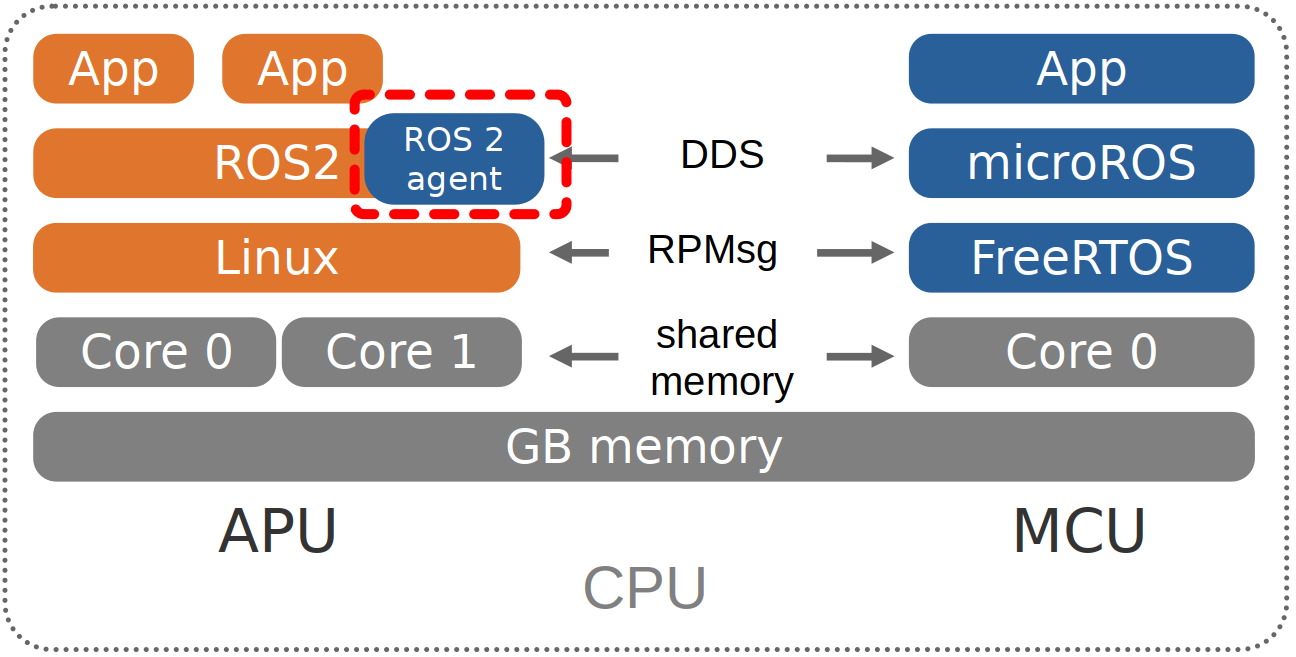
\includegraphics[width=.6\textwidth]{./img/map_agent.png}
\caption{\label{fig:org6b73f42}The agent (red border) allows for a micro-ROS instance to communicate with a ROS2 system. It is deployed on the Linux side, as a ROS2 node.}
\end{figure}

\subsection{Building a XRCE-DDS agent in a Docker}
\label{sec:org5e8e7d7}
The same command presented above for running a custom agent "bare-metal" can be
run inside a Docker.

\begin{minted}[frame=single,framesep=2mm,baselinestretch=1.2,linenos,breaklines,fontsize=\footnotesize]{sh}
docker run -d --name XRCE_DDS_Agent -it --net=host -v \
       /dev:/dev --privileged ros:iron
docker exec -it XRCE_DDS_Agent bash
\end{minted}


\begin{minted}[frame=single,framesep=2mm,baselinestretch=1.2,linenos,breaklines,fontsize=\footnotesize]{sh}
git clone https://github.com/eProsima/Micro-XRCE-DDS-Agent.git
cd Micro-XRCE-DDS-Agent
docker build -t xrce-dds-agent .
docker run -it --privileged -v /dev:/dev xrce-dds-agent serial \
       --dev /dev/ttyACM0
\end{minted}

\begin{minted}[frame=single,framesep=2mm,baselinestretch=1.2,linenos,breaklines,fontsize=\footnotesize]{sh}
git clone https://github.com/eProsima/Micro-XRCE-DDS-Agent.git
cd Micro-XRCE-DDS-Agent
docker build -t xrce-dds-agent .
docker run -it --privileged -v /dev:/dev xrce-dds-agent serial \
       --dev /dev/ttyACM0
\end{minted}

\section{Talker / ping-pong node\hfill{}\textsc{WORK\_IN\_PROGRESS}}
\label{sec:org50163a1}
A custom ping-pong node for ROS2 was developed in order to test the data transfer of the newly created
Agent / Client system.

In order to have this node up and running, you need to set basically all the previously presented points:
\begin{itemize}
\item On the same Linux you plan to run the node, you will need to run and keep the Agent, as presented
in the section \ref{sec:org7e1acf4}.
\item This ping-pong application is released as a ROS2 Python node. It is best to pull and run it
in a ROS2 environment to avoid having dependencies issues, as presented in the section about ROS2.

\clearpage
\end{itemize}
\section{Monitoring and performances evaluation\hfill{}\textsc{WORK\_IN\_PROGRESS}}
\label{sec:org76033c2}

\clearpage
\section{Conclusion \& future\hfill{}\textsc{WORK\_IN\_PROGRESS}}
\label{sec:org1ca591c}

\clearpage
\section{Publications\hfill{}\textsc{WORK\_IN\_PROGRESS}}
\label{sec:org331feca}
Tryna link the conference and journal paper related to this project here. Unclear how atm.

\clearpage
\appendix
\section{DTO patch}
\label{sec:orgb68d622}
This file is available in this repository: \href{https://gitlab.com/sunoc/xilinx-kria-kv260-documentation/-/blob/b7300116e153f4b5a1542f8804e4646db8030033/src/system.patch}{system.patch}
\inputminted[linenos, frame=single]{diff}{./src/system.patch}

\clearpage
\section{Custom tool-chain CMake settings}
\label{sec:org2dcb9ad}
This file is available in this repository: \href{https://gitlab.com/sunoc/xilinx-kria-kv260-documentation/-/blob/b7300116e153f4b5a1542f8804e4646db8030033/src/custom\_r5f\_toolchain.cmake}{custom r5f toolchain.cmake}
\inputminted[linenos, frame=single]{cmake}{./src/custom_r5f_toolchain.cmake}

\clearpage
\section{Custom Colcon meta settings}
\label{sec:org00d6274}
This file is available in this repository: \href{https://gitlab.com/sunoc/xilinx-kria-kv260-documentation/-/blob/b7300116e153f4b5a1542f8804e4646db8030033/src/custom\_r5f\_colcon.meta}{custom r5f colcon.meta}
\inputminted[linenos, frame=single]{yaml}{./src/custom_r5f_colcon.meta}

\clearpage
\section{Firmware time functions}
\label{sec:orgd94707c}

\subsection{main}
\label{sec:orgf8c14f0}
This file is available in this repository: \href{https://gitlab.com/sunoc/xilinx-kria-kv260-documentation/-/blob/b7300116e153f4b5a1542f8804e4646db8030033/src/clock.c}{clock.c}
but a potentially more up-to-date version is visible
directly at the \texttt{libmicroros\_kv260} repository: \href{https://gitlab.com/sunoc/libmicroros\_kv260/-/blob/4867e762f66af7b4647232eb4c0a31106db66e13/src/clock.c}{clock.c}

\inputminted[linenos, frame=single]{c}{./src/clock.c}

\subsection{header file}
\label{sec:org1cd3078}
\begin{minted}[frame=single,framesep=2mm,baselinestretch=1.2,linenos,breaklines,fontsize=\footnotesize]{c}
/**< Microseconds per second. */
#define MICROSECONDS_PER_SECOND    ( 1000000LL )  
/**< Nanoseconds per second. */
#define NANOSECONDS_PER_SECOND     ( 1000000000LL ) 
/**< Nanoseconds per FreeRTOS tick. */  
#define NANOSECONDS_PER_TICK       ( NANOSECONDS_PER_SECOND / configTICK_RATE_HZ ) 
\end{minted}


\clearpage
\section{Firmware memory allocation functions}
\label{sec:orgec8bbb4}

\subsection{main}
\label{sec:org7acd472}
This file is available in this repository: \href{https://gitlab.com/sunoc/xilinx-kria-kv260-documentation/-/blob/b7300116e153f4b5a1542f8804e4646db8030033/src/allocators.c}{allocators.c}
but a potentially more up-to-date version is visible
directly at the \texttt{libmicroros\_kv260} repository: \href{https://gitlab.com/sunoc/libmicroros\_kv260/-/blob/4867e762f66af7b4647232eb4c0a31106db66e13/src/allocators.c}{allocators.c}

\inputminted[linenos, frame=single]{c}{./src/allocators.c}

\subsection{header file}
\label{sec:org9691c14}
\begin{minted}[frame=single,framesep=2mm,baselinestretch=1.2,linenos,breaklines,fontsize=\footnotesize]{c}
#ifndef _ALLOCATORS_H_
#define _ALLOCATORS_H_

#include "microros.h"

extern int absoluteUsedMemory;
extern int usedMemory;


void * __freertos_allocate(size_t size, void * state);
void __freertos_deallocate(void * pointer, void * state);
void * __freertos_reallocate(void * pointer, size_t size, void * state);
void * __freertos_zero_allocate(size_t number_of_elements,
                                size_t size_of_element, void * state);

#endif // _ALLOCATORS_H_
\end{minted}
\section{[deprecated] Installing Linux (PetaLinux option)}
\label{sec:orgcad79e0}
This part is an alternative to the previous section \ref{sec:org8942216},
where the installation of PetaLinux as a host system\footnote{It is to be noted that for this part, the "other" KRIA board (KR260) was
used instead of the KV260 that was being used for everything tried on top of
Ubuntu. No significant difference should be noted.} will be presented,
as being an alternative to the Ubuntu LTS. Here are some reasoning why you'd
prefer to use PetaLinux instead of Ubuntu:
\begin{itemize}
\item Direct support from Xilinx. While Ubuntu is also an official port, it is
provided through Canonical.
\item If you plan to use ROS2 in containers.
\end{itemize}

It is also to be noted that the building process of a PetaLinux image is not as
trivial as simply flashing a downloaded ISO file. It takes some time to
configure it and even more time to be built, especially if you are working on a
lower-end machine.

\subsection{General installation}
\label{sec:orgb0aa5ec}
The indication on how to install PetaLinux on a KRIA board is detailed in the
official documentation\footnote{\url{https://xilinx.github.io/kria-apps-docs/kv260/2021.1/build/html/docs/build\_petalinux.html}}, but for the KV260 board with an older release of
the Linux. This guide will try to keep an up-to-date version of the guide, in
particular for the KR260 KRIA board and, at the time of writing, the PetaLinux
in version 2023.2 for the installer.  The 2022.2 version is recommended for this
board's latest updated boot firmware, as presented in the Section Boot firmware
above; however I happened to have issues with the building process from a system
based on Ubuntu 22.04. Thus the choice of the 2023.2 that should be compatible.

Two tools should be downloaded upfront in order to be ready and create the
PetaLinux image for our target board. Both can be obtained at the Xilinx
official download page\footnote{\url{https://www.xilinx.com/support/download/index.html/content/xilinx/en/downloadNav/embedded-design-tools/2022-2.html}}. Login with an AMD account is required in order to
download the files we need, namely, we'll have to get:
\begin{itemize}
\item The installer tool: \texttt{petalinux-v2023.2-10121855-installer.run} or similar name.
\item The SOM board support package: \texttt{xilinx-kr260-starterkit-v2023.2-10140544.bsp} or similar name\footnote{As of the time of writing this section, it was recommended\footnotemark to be
using the boot firmware in version 2022.2. Thus the software pack for the board
will also be using this version.}\footnotetext[32]{\label{org5a155c5}\url{https://xilinx-wiki.atlassian.net/wiki/spaces/A/pages/1641152513/Kria+SOMs+Starter+Kits\#K26-Boot-Firmware-Updates}}.
\end{itemize}
The specific name of the utils you'll get to download will evolve over time.

For the following command, I will assume that both files were downloaded into
the same directory and that you have a shell open in said directory.

Firstly, a crap ton of dependencies are needed. They are detailed in the
release notes of the version of the tool you are downloading and it depends on
your distribution, but here is a one-liner that works for the PetaLinux 2023.2
to be built on Ubuntu(-based) 22.04 LTS:
\begin{minted}[frame=single,framesep=2mm,baselinestretch=1.2,linenos,breaklines,fontsize=\footnotesize]{sh}
sudo apt-get install iproute2 gawk python3 build-essential gcc git make \
     net-tools libncurses5-dev tftpd zlib1g-dev libssl-dev flex bison libselinux1 \
     gnupg wget git-core diffstat chrpath socat xterm autoconf libtool tar unzip \
     texinfo zlib1g-dev gcc-multilib automake zlib1g:i386 screen pax gzip cpio \
     python3-pip python3-pexpect xz-utils debianutils iputils-ping python3-git \
     python3-jinja2 libegl1-mesa libsdl1.2-dev pylint asciidoc
\end{minted}

Testing, if building on Debian 12 the following variant of the same command has been confirmed to work:
\begin{minted}[frame=single,framesep=2mm,baselinestretch=1.2,linenos,breaklines,fontsize=\footnotesize]{sh}
sudo apt-get install iproute2 gawk python3 build-essential gcc git make \
net-tools libncurses5-dev tftpd-hpa zlib1g-dev libssl-dev flex bison libselinux1 \
gnupg wget git-core diffstat chrpath socat xterm autoconf libtool tar unzip \
texinfo zlib1g-dev gcc-multilib automake zlib1g screen pax gzip cpio python3-pip \
python3-pexpect xz-utils debianutils iputils-ping python3-git python3-jinja2 \
libegl1-mesa libsdl1.2-dev pylint asciidoc
\end{minted}

Installing the petalinux tools can be done with the \texttt{.run} script\footnote{It is to be noted that the \texttt{source} command will run best on \texttt{bash}. Trying
to run it on \texttt{zsh} for ex. will cause issues. This can be enforced with the
command \texttt{sudo dpkg-reconfigure bash}.}, as follow:
\begin{minted}[frame=single,framesep=2mm,baselinestretch=1.2,linenos,breaklines,fontsize=\footnotesize]{sh}
sudo chmod +x ./petalinux-v2023.2-10121855-installer.run
./petalinux-v2023.2-10121855-installer.run
bash
source settings.sh
\end{minted}

A project can then be created, using the \texttt{.bsp} file. From there it is possible to
build the image file meant to be booted by the board:
\begin{minted}[frame=single,framesep=2mm,baselinestretch=1.2,linenos,breaklines,fontsize=\footnotesize]{sh}
petalinux-create -t project -s xilinx-kr260-starterkit-v2023.2-10140544.bsp
cd xilinx-kr260-starterkit-2023.2/
\end{minted}


The more general option allows to enable stuff related to hardware
configuration\footnote{If you search in the work directory, you might notice that three
differently named \texttt{.xsa} files exist. After a quick \texttt{diff} check, they appear to be
exactly identical.}. For this step, it is possible to select the \texttt{openAMP}
setting the the DTG Settings, as visible in the Figure \ref{fig:org921f97a} below:
\begin{minted}[frame=single,framesep=2mm,baselinestretch=1.2,linenos,breaklines,fontsize=\footnotesize]{sh}
petalinux-config --get-hw-description  ./hardware/xilinx-kr260-starterkit-2023.2/kr260_starter_kit.xsa
\end{minted}

Then, here are the options that we want to enable:
\begin{figure}[htbp]
\centering
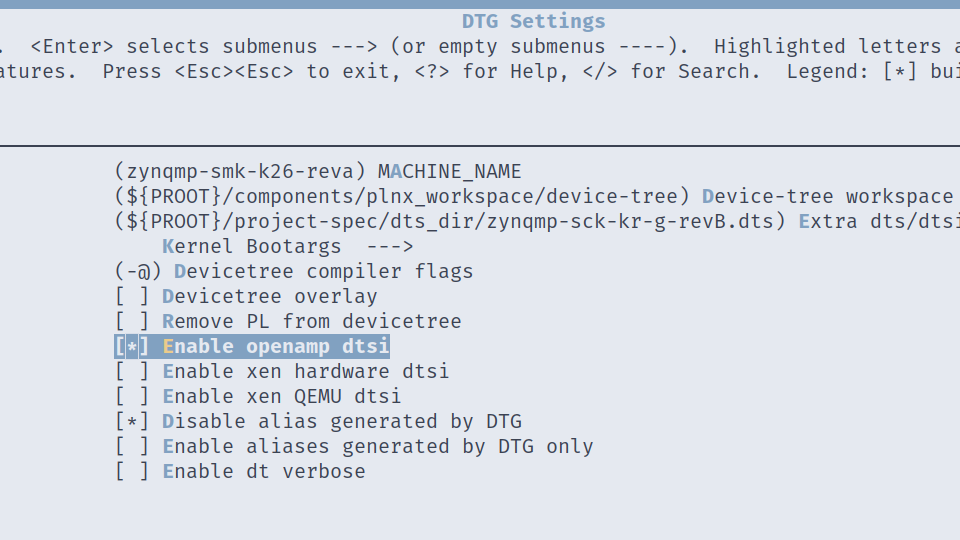
\includegraphics[width=.6\textwidth]{./img/yocto_openamp_dtg.png}
\caption{\label{fig:org921f97a}In the hardware config, it is possible to select the openamp device tree source.}
\end{figure}

Some kernel and module configuration are needed in order for the petalinux system to work properly.
These setup can be set using the following command:
\begin{minted}[frame=single,framesep=2mm,baselinestretch=1.2,linenos,breaklines,fontsize=\footnotesize]{sh}
petalinux-config -c rootfs
\end{minted}

Then, here are the options that we want to enable:
\begin{figure}[htbp]
\centering
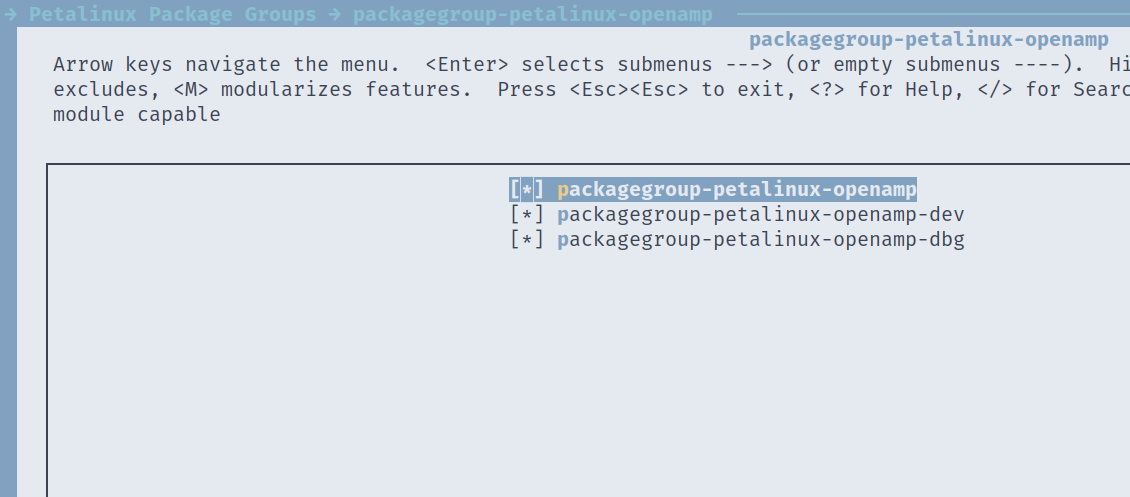
\includegraphics[width=.6\textwidth]{./img/yocto_openamp.png}
\caption{\label{fig:org3f1d85b}In the rootfs config, it is possible to select the openamp package.}
\end{figure}


\begin{figure}[htbp]
\centering
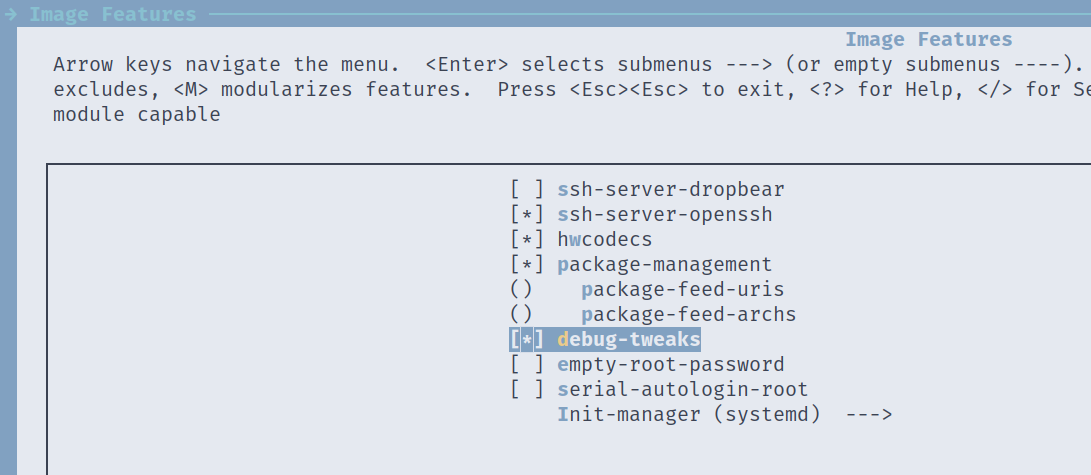
\includegraphics[width=.6\textwidth]{./img/yocto_ssh.png}
\caption{\label{fig:orgb08b280}OpenSSH can be configure in the same rootfs config.}
\end{figure}

It is then possible to build\footnote{Beware, the \texttt{petalinux-build} command execution takes a lot of time.} and package the image. Most critically compared to the example,
the \texttt{openamp.dtb} overlay must be used in order for OpenAMP and subsequently RPMsg to become usable.
\begin{minted}[frame=single,framesep=2mm,baselinestretch=1.2,linenos,breaklines,fontsize=\footnotesize]{sh}
petalinux-build
petalinux-package --wic --bootfiles "ramdisk.cpio.gz.u-boot boot.scr Image system.dtb"
\end{minted}

\begin{tcolorbox}[colback=red!5!white,colframe=red!75!black]
\textbf{DANGER}: The next part involve the \texttt{dd} command writing on disks!!!
As always with the dd command, thou have to be \textbf{VERY} careful on what arguments
thou give. Selecting the wrong disk will result on the destruction of
thy data !!
\uline{If you are unsure of what to do, seek assistance !}
\end{tcolorbox}

Finally, and now an image has been generated, it can be burnt to a micro-SD card the usual way:
\begin{minted}[frame=single,framesep=2mm,baselinestretch=1.2,linenos,breaklines,fontsize=\footnotesize]{sh}
sudo dd if=./images/linux/petalinux-sdimage.wic \
     of=/dev/sda status=progress bs=8M && sync
\end{minted}

From that point, the media can be ejected, put in the board and the boot process
should happen successfully.

\subsection{First login}
\label{sec:orgd7c9f7b}
On the first start, if you have a serial terminal open to the KR260 board, you'll be prompter to enter a login.
The default user it \texttt{petalinux}. You'll then be prompted to enter a password.

\subsection{Testing openamp "echo-test"}
\label{sec:org8d52ade}
A good and out-of-the-box way to try and confirm that the OpenAMP setup was done
properly is to run the so-called "echo-test". This program will basically send
series of packages to the R5F core and expect them to be returned.

As presented in the official documentation\footnote{\url{https://xilinx.github.io/kria-apps-docs/openamp/build/html/openamp\_landing.html\#openamp-demos}}, this can be simply done with
the following commands. If the return of the \texttt{echo\_test} commands states that zero
error occurs, the system should be good to go:
\begin{minted}[frame=single,framesep=2mm,baselinestretch=1.2,linenos,breaklines,fontsize=\footnotesize]{sh}
sudo -s
echo image_echo_test  > /sys/class/remoteproc/remoteproc0/firmware
echo start > /sys/class/remoteproc/remoteproc0/state
echo_test
echo stop > /sys/class/remoteproc/remoteproc0/state
\end{minted}

\subsection{"echo-test" performance comparison}
\label{sec:orgab4af82}

Now we have a working demonstration for RPMsg, a goal was to compare this system between boards.

Here is the complete sequence in order to archive a timely measured \texttt{echo\_test} run, namely:
\begin{itemize}
\item Installation of the build dependencies
\item Clone of the Xilinx repository
\item Patching of the main source to add the time measurement
\item Building of the test software
\item Communication with the R5F, with reload of the firmware
\end{itemize}
\begin{minted}[frame=single,framesep=2mm,baselinestretch=1.2,linenos,breaklines,fontsize=\footnotesize]{sh}
sudo dnf install git make gcc binutils packagegroup-core-buildessential
sudo ln -s /usr/bin/aarch64-xilinx-linux-gcc /bin/cc
git clone https://github.com/OpenAMP/openamp-system-reference.git
cd openamp-system-reference/examples/linux/rpmsg-echo-test/
wget https://gitlab.com/sunoc/xilinx-kria-kv260-documentation/-/raw/main/src/echo_test.patch
patch -u -b echo_test.c -i echo_test.patch
make
sudo -s
echo image_echo_test  > /sys/class/remoteproc/remoteproc0/firmware
echo start > /sys/class/remoteproc/remoteproc0/state
./echo_test
echo stop > /sys/class/remoteproc/remoteproc0/state
\end{minted}


The figure \ref{fig:orgb8d0ede} below shows a comparison for the data
throughput that is reachable for a packages round trip of individual RPMsg
packages for both PetaLinux running on the KR260 board and Ubuntu running on the
KV260.

A difference exist but it is not as significant as to explain the rather slow
transfer rate when used in combination with ROS2 DDS.

\begin{figure}[htbp]
\centering
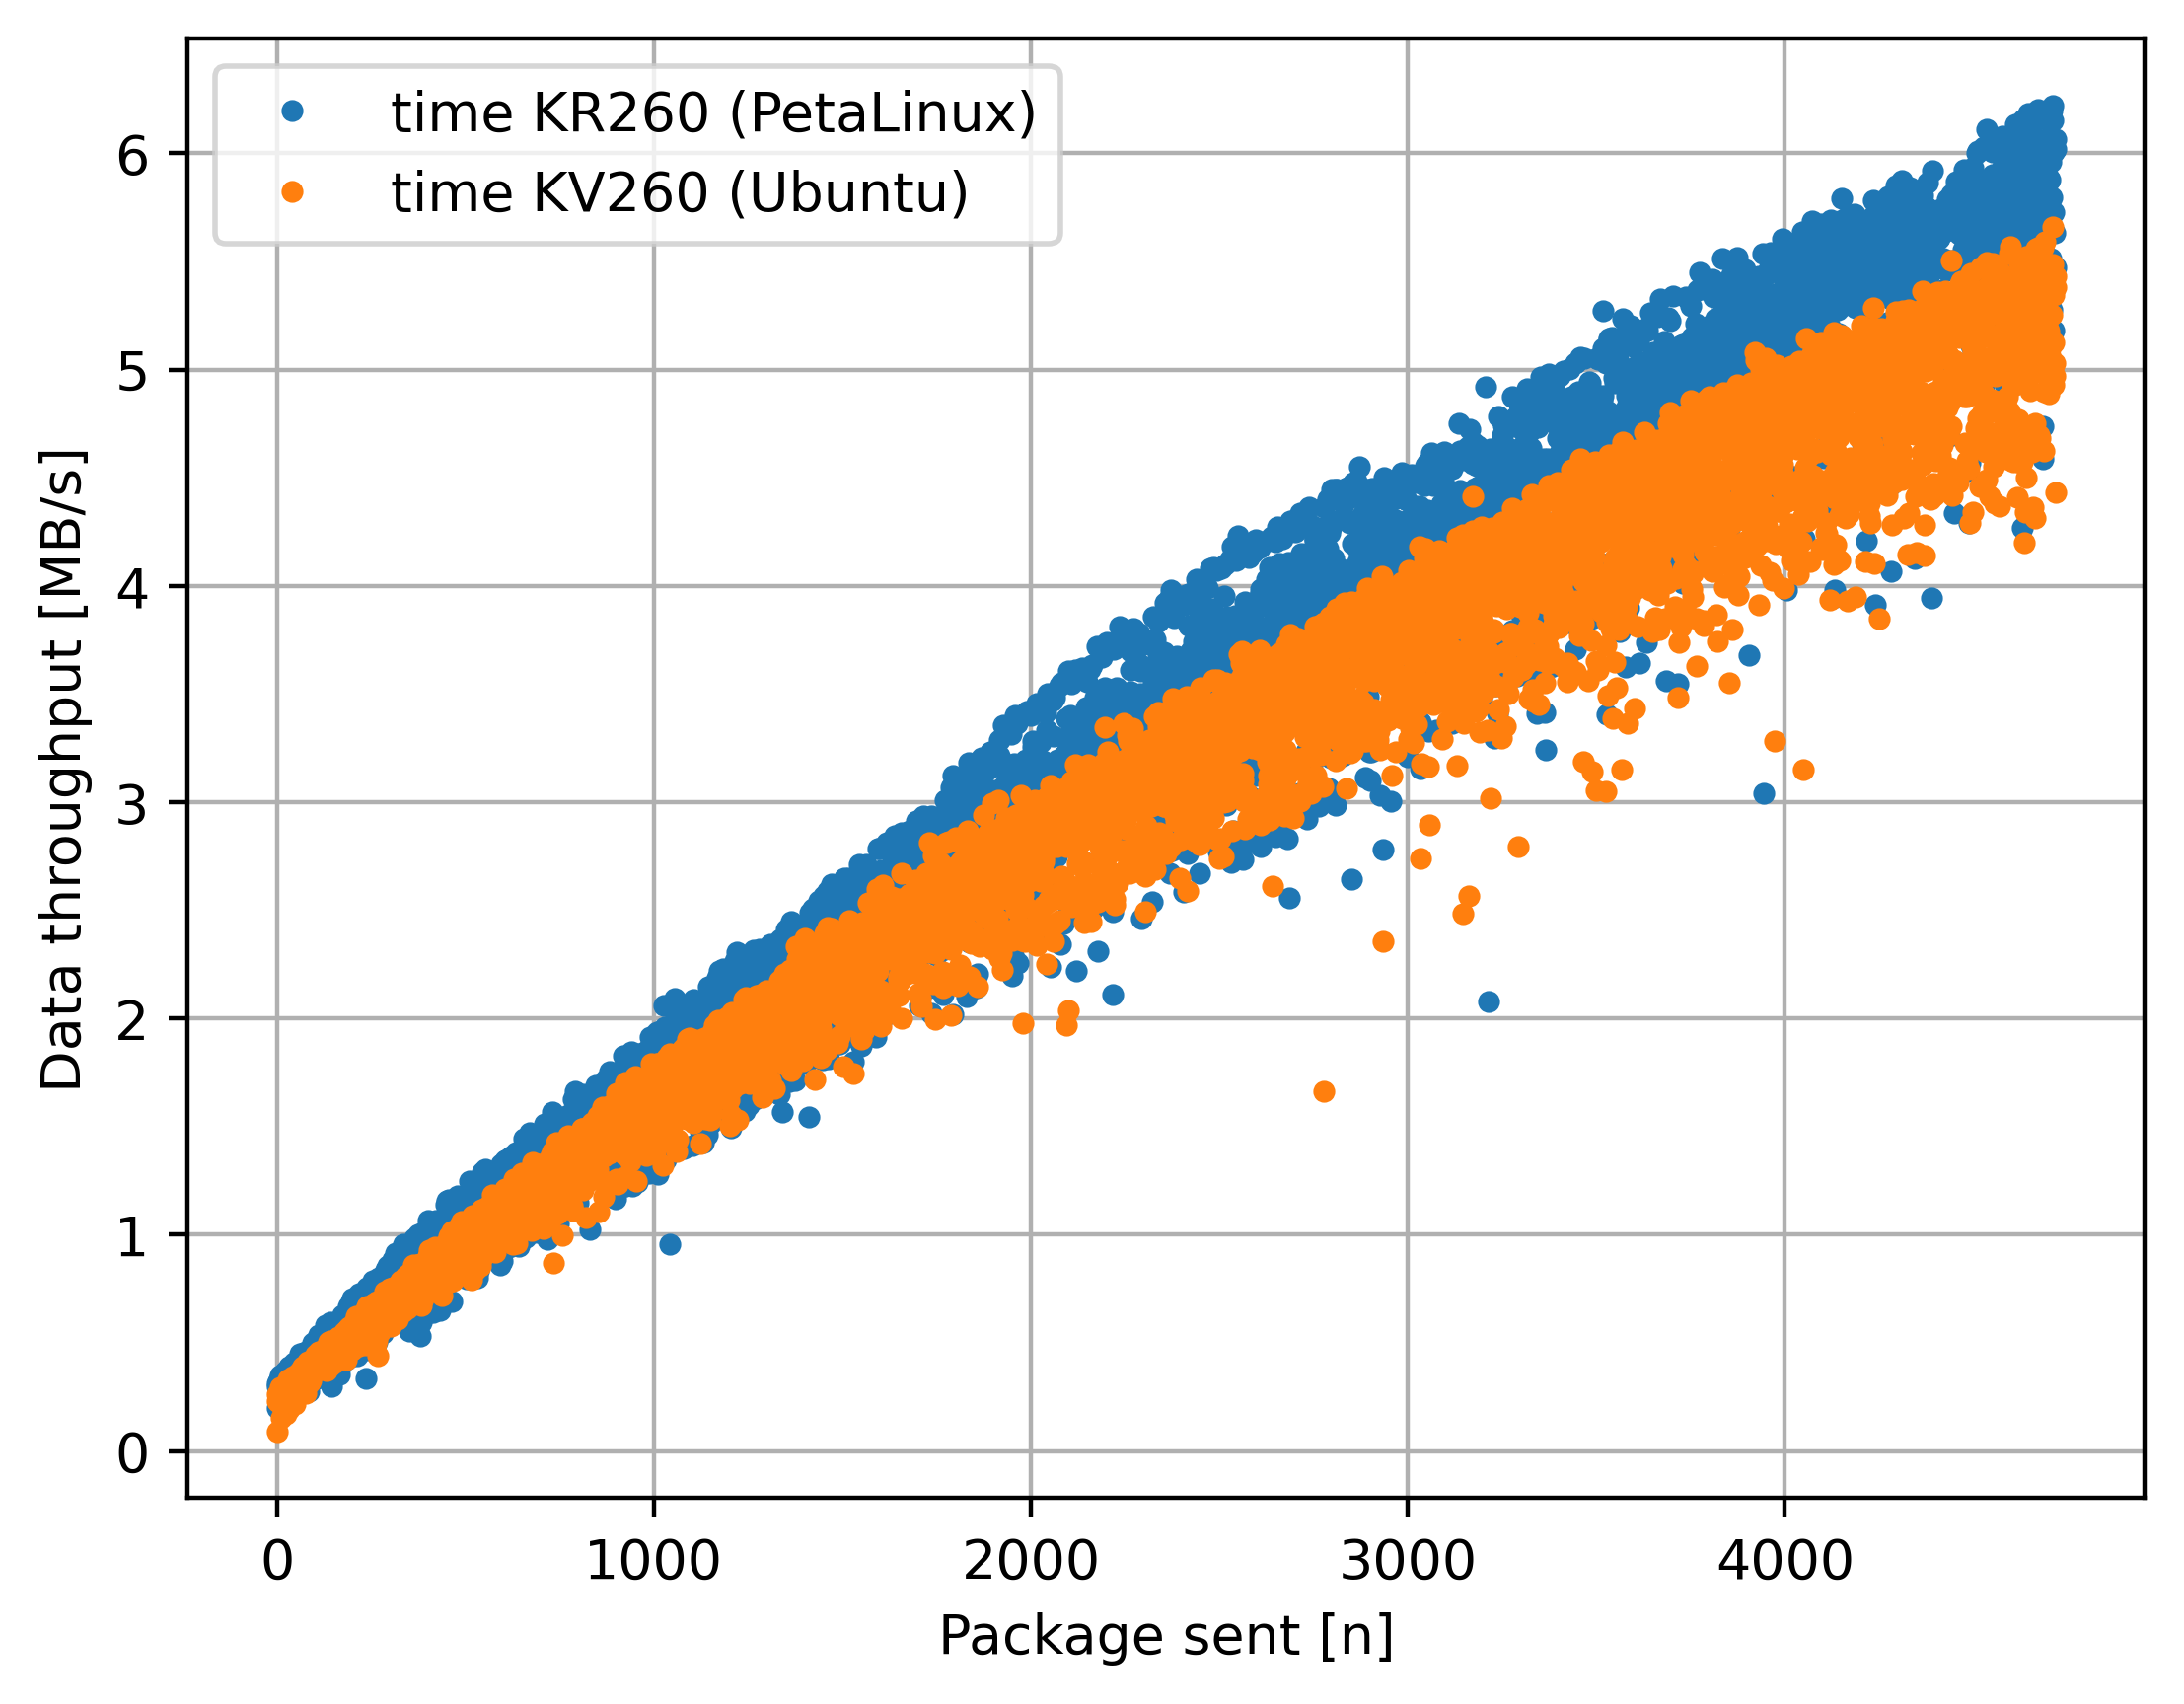
\includegraphics[width=.6\textwidth]{./img/kr260_echo_test_density.png}
\caption{\label{fig:orgb8d0ede}A graph of the data transfer rate for individual packages to be transmitted and received back from the Linux.}
\end{figure}

This fast delay for data transmission was later confirmed by measurement done using an external logic analyser\footnote{\url{https://gitlab.com/sunoc/saleae-logic-8-documentation}}.

\subsection{Enabling SSH}
\label{sec:orge1b0888}
\subsection{Setting up a static IP address for PetaLinux}
\label{sec:org1ea6f3b}
This is not a trivial task in petalinux.

As it appears, the classic \texttt{/etc/network/interfaces} must be modified, however and
for some unknown reason the DHCP keep being used even when disabled, and the
actual static interface is not used until restarted.

Multiple steps are required in order to mitigate all of this.

First, we can make our standard \texttt{interfaces} configuration, in the  \texttt{/etc/network/interfaces}:
\begin{minted}[frame=single,framesep=2mm,baselinestretch=1.2,linenos,breaklines,fontsize=\footnotesize]{sh}
# Wired or wireless interfaces
auto eth0
iface eth0 inet static
address 192.168.11.107
netmask 255.255.255.0
network 192.168.11.0
gateway 192.168.11.1
\end{minted}

Then we need to have \texttt{systemd} to run a script after boot time to restart the \texttt{eth0} interface.

A very basic script, as follow need to be placed somewhere on the system, for example here, in the \texttt{/home/root/net.sh}:
\begin{minted}[frame=single,framesep=2mm,baselinestretch=1.2,linenos,breaklines,fontsize=\footnotesize]{sh}
#!/bin/sh -e
ifdown eth0
ifup eth0
exit 0
\end{minted}

Then, we want to create a \texttt{systemd} service that will run this script as \texttt{idle},
i.e. after all the rest. Said file, in our case named \texttt{updown.service} must be
placed in the \texttt{/etc/systemd/system/} directory:
\begin{minted}[frame=single,framesep=2mm,baselinestretch=1.2,linenos,breaklines,fontsize=\footnotesize]{yaml}
[Unit]
Description=Restart once more the eth0 network to enable the static IP

[Service]
Type=idle
ExecStart=/bin/sh /home/root/net.sh

[Install]
WantedBy=multi-user.target
\end{minted}

Finally, as a \texttt{root} we need to set the correct right for these files and finally enabling the service before reboot:
\begin{minted}[frame=single,framesep=2mm,baselinestretch=1.2,linenos,breaklines,fontsize=\footnotesize]{sh}
sudo -s
chmod +x /home/root/net.sh
chmod 644 /etc/systemd/system/updown.service
systemctl enable updown.service
reboot now
\end{minted}

With all of this, on the next reboot of the board, the static IP should be available alongside the DHCP IP.

\section{References}
\label{sec:org92a6565}
\bibliographystyle{ieeetr}
\bibliography{../../../Documents/Bibliography/references}
\end{document}
